%\chapter{Gravitational physics}
%
%The following section aims to develop concepts of gravitation that are present in Newton's theory of gravitation and play a fundamental role in the generation of gravitational waves in more modern theories such as general relativity.  It aims to motivate the importance of concepts such as EOS and multipole moments, followed by a simple introduction to Einstein's field equations and some applications relevant in GW astronomy.
%
%
%\section{Newtonian gravity}
%
%In the following, we will present the fundamentals of newton's theory of gravitation, with the aim of being able to speak of mass distributions more generalized than the case of point particles. In addition, motivated by the descriptions made in books by Shapiro\cite{Shapiro:1983du} and Poisson \cite{poisson_will_2014}, the classical example of a self gravitating degenerate fermi gas in hydrostatic equilibrum is presented in detail to later stablish the parallelism with its relativistic version.
%
%
%It is surprising how well Newtonian gravity reproduces the effects of systems in the presence of weak gravitational fields. For centuries astronomers were able to make predictions and confirm its versatility in systems such as main sequence stars, galaxies, the Earth-Moon system, and planets of the solar system (not without problems). For this reason, it is taken as a reference for more modern theories of gravity, which by convention are asked to reproduce its effects in the slow motion approximation,i.e., $\frac{||\vec{v}||}{c} << 1$ and weak field limit $\frac{GM}{c^2 R} <<1$. It is important to emphasize that it is an incomplete theory. Although it works quite well in the examples mentioned, it is unable to reproduce phenomena such as gravitational lensing, gravitational redshift and gravitational waves.
%
%Although Newton's work in gravitation is better known by the inverse square law, its description as a field theory via the Poisson's equation its more modern, and allow us to see directly its simplicity and to establish its differences with Einstein's field equations. Let us begin by writting down poisson's equation for gravitation  and it's solution in term's of green's functions 
%
%\begin{equation}\label{poisson}
%\nabla^2 \phi = -4\pi G \rho(t, \vec{x}).
%\end{equation}
%
%\begin{equation}\label{phi}
%\phi(t, \vec{x}) = -4\pi G \left( \frac{1}{4\pi} \int_{V} \frac{\rho(t, \vec{x}')}{|| \vec{x}-\vec{x}' ||} d^3x'\right).
%\end{equation}
%
%Where G is the gravitational constant. From which one can naturally define the active gravitational mass as the flux of the force field $\vec{g}=-\vec{\nabla} \phi(t, \vec{x}')$ and its flux throught the surface $\partial V$ 
%
%\begin{equation}
%dm(t, \vec{x}) = \frac{1}{4\pi G} \cdot \vec{\nabla}(\vec{\nabla}\phi) dV,
%\end{equation}
%
%\begin{equation}
%m(t, \vec{x}) = -\frac{1}{4\pi G}\int_{V} \vec{\nabla} \cdot (\vec{\nabla} \phi(t, \vec{x}')) d^3 x' ,
%\end{equation}
%
%\begin{equation}\label{active mass}
%m(t, \vec{x}) = \frac{1}{4\pi G}\int_{\partial V}  \vec{g}\cdot \hat{n}  \;\; d^2 x'.
%\end{equation}
%
%
%Where $\hat{n}$ represents the unit normal vector field to the surface $\partial V$. Solutions to equation \ref{phi}, together with newtown's second law, and an equation of state, allow us to compute interesting physical observables like the orbits of bodies in presence of the field $\phi$, the internal structure of self gravitating objects and their binding energy.
%
%
%In general, solutions to equation \ref{poisson} can be computed using analytical methods as in electromagnetism(see \cite{Jackson:1998nia}), numerical methods, or the multipole expansion (see for example \cite{Thorne:1980ru}). The later being a powerful tool to perform analitical calculations on complicated geometries. It has also been used in experiments on the solar sistem, and to measure earth's surface potential \cite{GOCE, GRACE}. 
%
%
%\subsection{The multipole expansion}
%
%Series expansions are a systematic tool for working with gravitational fields produced by generalized mass distributions. Analytical calculations and gravitational physics experiments both in laboratories and in Earth orbit often use spherical coordinates and decompose the function $\frac{\alpha}{||\vec{x}-\vec{x'}||}$ in terms of its spherical harmonics \cite{Muller,kaula1966theory,Stirling:2017ybn}. However, the derivation of the multipole expansion will be presented below in Cartesian coordinates to match the conventions of the gravitational wave section in the books by Hartle \cite{Hartle:2021pel} and Creighton et al. \cite{Creighton:2011zz}.
%
%Let us begin by enumerating the following identity for the Taylor expansion of a scalar function $f$.
%
%
%\begin{equation}
%f(x') = f(x')\Biggr|_{\vec{x'_0}} + ((x-x'_0)\cdot \nabla) f(x)\Biggr|_{\vec{x'_0}} + \frac{1}{2!} ((x-x'_0)\cdot \nabla)((x-x'_0)\cdot \nabla) f(x)\Biggr|_{\vec{x'_0}} + ...
%\end{equation}
%
%Which can also be expressed by components using a Cartesian orthonormal basis $\theta^a:= {\hat{i}, \hat{j},\hat{k}}$ . In these terms, the differential operator $\nabla$ becomes $\frac{\partial}{\partial x^a} \theta^a$ and the vector $(x-x'_0)$ can be rewritten as $(x - x'_0)^b e_b$. Where $e_b$ is the dual basis given by $\theta^a e_b= \delta^a_b$
%
%%\begin{equation}
%\begin{multline}
%f(x'^a) = f\Biggr|_{\vec{x'_0}} + \left( \frac{\partial f}{\partial x'^a} \theta^a \right)\Biggr|_{\vec{x'_0}} (x' - x'_0)^b e_b \\ + \frac{1}{2!} \left( \frac{\partial^2 f}{\partial x'^a \partial x'^b} \theta^a \otimes \theta^b \right)\Biggr|_{\vec{x'_0}} (x' - x'_0)^c e_c (x' - x'_0)^d e_d + ...\;\; ,
%\end{multline}
%%\end{equation}
%
%\begin{equation}\label{tay.exp}
%f(x'^a) = f\Biggr|_{\vec{x'_0}} + \left( \frac{\partial f}{\partial x'^a} \right)\Biggr|_{\vec{x'_0}} (x' - x'_0)^b \delta^a_b + \frac{1}{2!} \left( \frac{\partial^2 f}{\partial x'^a \partial x'^b}  \right)\Biggr|_{\vec{x'_0}} (x' - x'_0)^c  (x' - x'_0)^d \delta^a_d \delta^b_d +   ... \;\; ,
%\end{equation}
%
%\begin{multline}
%\left( \frac{1}{|| \vec{x} - \vec{x}'||} \right) = \left( \frac{1}{|| \vec{x} - \vec{x}'||} \right)\Biggr|_{\vec{x'_0}} + \left( \frac{\partial \left( \frac{1}{|| \vec{x} - \vec{x}'||} \right)}{\partial x'^a} \right)\Biggr|_{\vec{x'_0}} (x' - x'_0)^b \delta^a_b \\+ \frac{1}{2!} \left( \frac{\partial^2 \left( \frac{1}{|| \vec{x} - \vec{x}'||} \right)}{\partial x'^a \partial x'^b}  \right)\Biggr|_{\vec{x'_0}} (x' - x'_0)^c  (x' - x'_0)^d \delta^a_d \delta^b_d + ... \;\;.
%\end{multline}
%
%
%Now, let's apply the expansion \ref{tay.exp} to the function $\frac{1}{||\vec{x}-\vec{x'}||}$. To do this, we first write its denominator in components and calculate its first and second derivatives:
%
%$$ \frac{1}{|\vec{x}-\vec{x'}|} \rightarrow \frac{1}{(\delta_{ab} (x- x')^a (x- x')^b)^\frac{1}{2}}$$
%
%\begin{equation}\label{first der.}
%\frac{\partial}{\partial x'^a}(\delta_{cd} (x- x')^c (x- x')^d)^{-\frac{1}{2}} = \frac{(x_a - x'_a)}{(\delta_{cd} (x- x')^c (x- x')^d)^{\frac{3}{2}}} \;\; ,
%\end{equation}
%
%\begin{multline}\label{second der.}
%\frac{\partial^2}{\partial x'^a \partial x'^b}(\delta_{cd} (x- x')^c (x- x')^d)^{-\frac{1}{2}} = \frac{-\delta_{ab}}{(\delta_{cd} (x- x')^c (x- x')^d)^{\frac{3}{2}}}\\ +\frac{3(x_a - x'_a)(x_b - x'_b)}{ (\delta_{cd} (x- x')^d (x- x')^d)^{\frac{5}{2}} } \;\; .
%\end{multline}
%
%
%Inserting  \ref{first der.} and \ref{second der.} into the first two terms of the expansion \ref{tay.exp}, and taking $\vec{x}_0 = \vec{0}$, the expansion becomes: 
%
%\begin{equation}
%\left( \frac{1}{|| \vec{x} - \vec{x}'||} \right) = \left( \frac{1}{|| \vec{x}||} \right) + \frac{x_a x'^b \delta^a_b}{||\vec{x}||^3} + \frac{1}{2!} \left(\frac{-\delta_{ab}}{||\vec{x}||^3} + \frac{3 x_a x_b}{||\vec{x}||^5}  \right) x'^c x'^d \delta^a_c \delta^b_d +  ... \;\; ,
%\end{equation}
%
%
%\begin{equation}
%\left( \frac{1}{|| \vec{x} - \vec{x}'||} \right)(x'^a) = \left( \frac{1}{r} \right) + \frac{n_a x'^a}{r^2} + \\ \frac{1}{2!} \left(\frac{ 3 n_a n_b -\delta_{ab}}{r^3}  \right) x'^a x'^b + O(r^{-4})\;\; .
%\end{equation}
%
%
%Where $r = ||\vec{x}||$ and $n_a = \frac{x_a}{r}$. We truncate the series on the third term, so that the gravitational potential \ref{phi} 
%
%\begin{equation}\label{multipole0}
%\phi(t, \vec{x}) = -G \int_{\Omega} d^3x' \rho(t, \vec{x}) \left[ \frac{1}{r} + \frac{n_a x'^a}{r^2} + \frac{1}{2} \left( \frac{ 3 n_a n_b -\delta_{ab} }{r^3}  \right) x'^a x'^b \right]
%\end{equation}
%
%
%\begin{equation}\label{multipole1}
%\phi(t, \vec{x}) = -G \left[ \frac{\mathcal{M}}{r} + \frac{n_a \mathcal{D}^a}{r^2} + \frac{1}{2} \frac{ \left( 3 n_a n_b -\delta_{ab} \right) \mathcal{Q}^{ab} }{r^3} \right]
%\end{equation}
%
%$\mathcal{M}$, $\mathcal{D}^a$ and $\mathcal{Q}^{ab}$ are called monopole, dipole and quadrupole moments respectively
%
%\begin{equation}
%\mathcal{M} := \int_{\Omega} d^3x' \;\; \rho(t, \vec{x}'),
%\end{equation}
%
%
%\begin{equation}
%\mathcal{D}^a := \int_{\Omega} d^3x' \;\; x'^a \rho(t, \vec{x}'),
%\end{equation}
%
%
%\begin{equation}\label{quadrupole}
%\mathcal{Q}^{ab} := \int_{\Omega} d^3 x' \;\;x'^a x'^b \rho(t, \vec{x}).
%\end{equation}
%
%
%%\textit{Remark}: one can always rewrite the third term by adding a traceless extra term, for example, $-r^2 \delta^{ab}$ 
%%
%%$$
%%\left( n_a n_b - \frac{1}{3} \delta_{ab}\right) \left( 3 x'^a x'^b - r^2\delta^{ab} \right) = \left( n_a n_b - \frac{1}{3} \delta_{ab} \right) 3 x'^a x'^b - r^2 \delta^{ab} (n_a n_b - \frac{1}{3} \delta_{ab})
%%$$
%%
%%$$
%%\left( n_a n_b - \frac{1}{3} \delta_{ab}\right) \left( 3 x'^a x'^b - r^2\delta^{ab} \right) = \left( n_a n_b - \frac{1}{3} \delta_{ab}\right) 3 x'^a x'^b - \cancel{r^2 (1-1)}
%%$$
%%
%%So that the gravitational potential can be separated into monopole, dipole, and quadrupole moment contributions 
%%$$
%%\phi(t, \vec{x}) = -G \int_{\Omega} d^3x' \rho(t, \vec{x}) \left[ \frac{1}{r} + \frac{n_a x'^a}{r^2} + \frac{1}{2} \left( \frac{ \left( n_a n_b - \frac{1}{3} \delta_{ab}\right) \left( 3 x'^a x'^b - r^2\delta^{ab} \right) }{r^3}  \right) \right]
%%$$
%%
%%$$
%%\phi(t, \vec{x}) = -G \int_{\Omega} d^3x' \rho(t, \vec{x}) \left[ \frac{1}{r} + \frac{n_a x'^a}{r^2} + \frac{1}{2} \frac{ \left( n_a n_b - \frac{1}{3} \delta_{ab}\right) \left( 3 x'^a x'^b - r^2\delta^{ab} \right) }{r^3} \right]
%%$$
%%
%%\begin{equation}\label{multipole1}
%%\phi(t, \vec{x}) = -G \left[ \frac{\mathcal{M}}{r} + \frac{n_a \mathcal{D}^a}{r^2} + \frac{1}{2} \frac{ \left( n_a n_b - \frac{1}{3} \delta_{ab}\right) \mathcal{Q}^{ab} }{r^3} \right]
%%\end{equation}
%%
%%
%%$$
%%\mathcal{M} := \int_{\Omega} d^3x' \;\; \rho(t, \vec{x}')
%%$$
%%
%%$$
%%\mathcal{D}^a := \int_{\Omega} d^3x' \;\; x'^a \rho(t, \vec{x}')
%%$$
%%
%%$$
%%\mathcal{Q}^{ab} := \int_{\Omega} d^3 x' \;\;x'^a x'^b \rho(t, \vec{x}) =  \int_{\Omega} d^3 x' \left( 3 x'^a x'^b - r^2\delta^{ab} \right) \rho(t, \vec{x}')
%%$$
%
%The quadrupole moment gets to be an extremely relevant quantity when studying extended bodies and tidal interactions. Given two neighouring particles, their separation vector $\vec{\xi}$ with components $\xi^i = \{\xi^x, \xi^y, \xi^z \} $ in presence of a gravitational field $\phi$, evolves acording to 
%
%
%\begin{equation}\label{tidal0}
%\frac{d^2 \xi^{i}}{dt^2} = - \left(\frac{\partial^2 \phi }{\partial x^j \partial x^i} \right) \xi^{j}.
%\end{equation} 
%
%It is coupled to the field \ref{multipole0} through its second derivatives, i.e., it is predominantly quadrupolar in nature.
%
%Equation \ref{quadrupole} contributes to the generation of ocean tides on Earth in the presence of the Moon's gravitational field \cite{Hartle:2021pel}. In addition, measurements of the Sun's quadrupole momentum have been crucial in helioseismology, and solar system physics. It also plays a fundamental role in the generation of gravitational waves in general relativity, since, as will be shown later, only sources with a time-varying quadrupole momentum emit gravitational radiation \cite{Creighton:2011zz}.
%
%\subsection{Spherically symmetric polytropic stars}
%
%The internal structure of self-gravitating systems like ideal white dwarfs, main sequence stars and in general systems with small compactness parameter are worth exploring in the Newtonian limit. Since their gravitational fields are very weak, their internal structure, properties and evolution are reproduced relatively well if a good matter model and microphysics are provided. The following table taken from the book of Shapiro and Teukolsky \cite{Shapiro:1983du} serves as a rough overview of the most compact objects observed to date, compared to the sun.
%\vspace{1cm}
%
%\begin{table}[!htbp]
%\begin{center}
%\begin{tabular}{ccccc}
%\hline\\
%object &Mass&Radius& Mean Density& Compactness parameter \\
%       & [$M_\odot$]& $[R_\odot]$& [Kg/$m^3$]& GM/R$c^2$  \\
%\hline \\
%Sun           &1          &1         &$\approx 10^{3}$   &$ 10^{-6}$ \\
%White dwarf   &$< 1.4$ &$10^{-2}$    &$< 10^{10}$        &$\approx 10^{-4}$ \\
%Neutron star  &1-3        &$10^{-5}$ &$< 10^{18}$        &$\approx 10^{-1}$ \\
%Black Hole    &Arbitrary  &2GM/$c^2$ & $\approx M/R^{3}$ & $\approx 1$ \\
%\hline
%\end{tabular}
%\captionsetup{width=.8\textwidth}
%\caption{Compact objects compared to the sun}
%\caption*{The information in this table was taken from \cite{Shapiro:1983du}. It lists rough upper bounds for masses, radii, and mean densities and ends by listing the compactness parameter for each object in the last column, also known as surface potential.}
%\label{compactness}
%\end{center}
%\end{table}
%
%The following is a derivation of the mass-radius relation for a non-rotating spherically symmetric mass distribution, in hydrostatic equilibrium. In addition the equation of state for an ideal degenerate fermi gas will be taken into account to show explicitly the process of obtaining several properties of ideal white dwarfs, as chandrasekhar did in his work \cite{Chandrasekhar:1931ih}. This subsection is also intended to give an idea of a case where the equations of hydrostatic equilibrium can be integrated analytically, as oposed to most cases in General relativity(see fig. \ref{equations of state and tidal deformability})
%
%Let us start by considering a spherically symmetric mass distribution of radius r, and take the effects of gravity on an infinitesimal mass element $dm$ occupying a volume $dV$. In spherical coordinates the mass as a function of the radial coordinate and its first derivative are given by
%
%% is $dV =  r^2 \sin(\phi) dr d\theta d\phi$, so that when integrating the mass distribution $\rho(r)$ the angular part gives the constant factor $4\pi$ 
%
%
%%\begin{figure}[hbt!]
%%\begin{center}
%%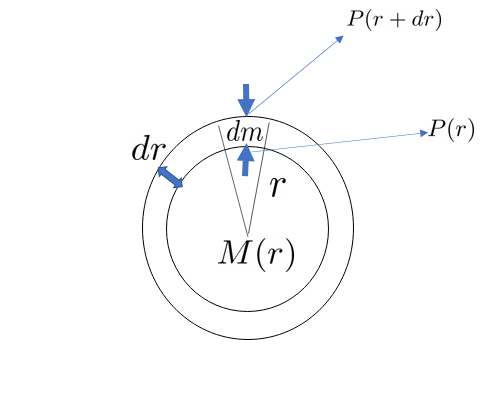
\includegraphics[width=0.5\textwidth, angle=0]{images/polytropes.png}
%%\caption{Spherically symmetric and static star}
%%\label{polytropes0}
%%\end{center}
%%Slice of a sphere along $\phi=constant$. The Inward pointing blue arrow is assigned to the gravitational force, and the outward pointing arrow to the pressure force exerted on the mass element $dm$.
%%\end{figure}
%%
%%\FloatBarrier
%
%
%\begin{equation}\label{mass}
%M(r) = 4\pi  \int_0^{r} dr' \;\; r'^2 \rho(r') 
%\end{equation}
%
%\begin{equation}\label{massprime}
%\frac{dM(r)}{dr} = 4\pi r^2 \rho(r) 
%\end{equation}
%
%To build such an object in an equilibrium configuration, one must require a balance between the outward-pointing force produced by the internal degeneracy pressure and the inward-pointing gravitational force produced by its weight 
%
%\begin{equation}\label{grav.f}
%\vec{F_p} = \delta P dS\;\; \hat{e}_r = - \left(P(r+dr) - P(r) \right)  r^2 \sin (\theta) d\theta d\phi \;\; \hat{e}_r, 
%\end{equation}
%
%\begin{equation}\label{press.f}
%\vec{F_g} = \frac{G M(r) dm(r)}{r^2} \;\; \hat{e}_r = \frac{G M(r) (\rho(r) r^2 \sin(\theta) dr d\theta d\phi)}{r^2} \;\; \hat{e}_r
%\end{equation}
%
%The hydrostatic equilibrium condition leads us to an expression of pressure gradient in terms of mass and the density at a certain distance r from its center.
%
%$$
%-\frac{dP}{dr} dr \cdot r^2 \sin(\theta) d\theta d\phi = \frac{G M(r) (\rho(r) r^2 \sin(\theta) dr d\theta d\phi)}{r^2}
%$$
%
%\begin{equation}\label{press.grad}
%-\frac{dP}{dr} = \frac{G M(r) \rho(r)}{r^2}, 
%\end{equation}
%
%However, equations \ref{massprime} and \ref{press.grad}, form an system of differential equations that has to be completed by a function that relates pressure and density to be integrated. It is called equation of state.
%
%\begin{equation}\label{lim.TOV2}
%P = P(\rho)
%\end{equation}
%
%Currently, realistic matter models encoded in realistic equations of state can be found in the literature as shown in figure \ref{equations of state and tidal deformability}, but one can not find closed-form solutions to equations \ref{lim.TOV0}, \ref{lim.TOV1} and \ref{lim.TOV2} using them.
%
%Nevertheless, polytropic equations of state \ref{EOS0} are simple enough to produce analytic results while still being good models for ideal stars \cite{Chandrasekhar:1931ih}. Their mass-radius relation can be written in straightforward terms and was widely explored by Chandrasekhar's work on ideal White dwarfs \cite{Shapiro:1983du,Chandrasekhar:1931ih, camenzind}. 
%
%\begin{equation}\label{EOS0}
%P = k \rho^{\Gamma} = k \rho^{\frac{n+1}{n}}
%\end{equation}
%
%\begin{equation}\label{EOS1}
%P' = k \Gamma \rho^{\Gamma-1} \rho'
%\end{equation}
%
%
%Where the prime means derivative with respect to the radial coordinate $r$, $\Gamma$ is called polytropic exponent, and $n$ polytropic index. One can insert equation \ref{EOS1} in equation \ref{lim.TOV0} to get only powers of the density and its derivatives on the left and the mass on the right-hand side. Further, one can get different solutions depending on the values of $\Gamma$. 
%
%$$
%-\left( \frac{k \Gamma r^2}{G} \right) \rho^{\Gamma-2} \rho' = M
%$$
%
%%An elementary ODE shows up after evaluating $\Gamma=1$ and then differentiating both sides.
%%
%%\begin{equation}
%%-\left( \frac{k}{G} \right) (r^2\rho^{-1} \rho')' = M' \rightarrow -\left( \frac{k}{G} \right) (r^2 \frac{\rho'}{\rho})' = 4\pi r^2 \rho
%%\end{equation}
%%
%%\begin{equation}
%% -\left( \frac{k}{4\pi G r^2} \right) (r^2 \frac{\rho'}{\rho})' = \rho
%%\end{equation}
%
%For $\Gamma \neq 1$, we use the identity $\rho^{\Gamma-2} \rho' = \frac{(\rho^{(\Gamma -1)})'}{(\Gamma -1)}$, and then differentiate both sides
%
%\begin{equation}
%-\left( \frac{k \Gamma}{G(\Gamma-1)} \right) (r^2 (\rho^{\Gamma-1})')' = M',
%\end{equation}
%
%multiply by $\frac{\rho_0^{\Gamma-1}}{\rho_0^{\Gamma-1}}$ on the left and then divide both sides by  the central densitiy $\rho_0 = \rho(r=0)$
%
%\begin{equation}
%-\left( \frac{k \Gamma}{4\pi G(\Gamma-1)} \right)\left(\frac{1}{r^2}\right) \left( \frac{\rho_0^{\Gamma-1}}{\rho_0^{\Gamma-1}} \right) \left( \frac{1}{\rho_0} \right)(r^2 (\rho^{\Gamma-1})' )' = \left( \frac{1}{\rho_0} \right) \rho \;\;,
%\end{equation}
%
%%\begin{equation}
%%-\left( \frac{k \Gamma}{4\pi G(\Gamma-1)} \right)\left(\frac{1}{r^2}\right) \left( \frac{\rho_0^{\Gamma-1}}{\rho_0^{\Gamma-1}} \right) \left( \frac{1}{\rho_0} \right)(r^2 (\rho^{\Gamma-1})' )' = \left( \frac{1}{\rho_0} \right) \rho\;\;,
%%\end{equation}
%
%\begin{equation}
%-\left( \frac{k \Gamma}{4\pi G(\Gamma-1)} \right)\left( \rho_0^{\Gamma-2} \right) \left(\frac{1}{r^2}\right) \frac{d}{dr} \left(r^2 {\frac{d}{dr}\left(\frac{\rho}{\rho_0}\right)}^{\Gamma-1} \right) =  \frac{\rho}{\rho_0}\;\;.
%\end{equation}
%
%After rearranging terms and doing algebra, we arrive at equation \ref{pre.lane-emden}
%
%%\begin{equation}
%%-\left( \frac{1}{\frac{4\pi G(\Gamma-1)}{k \Gamma \left( \rho_0^{\Gamma-2} \right)}} \right) \left(\frac{1}{r^2}\right) \frac{d}{dr} \left(r^2 {\frac{d}{dr}\left(\frac{\rho}{\rho_0}\right)}^{\Gamma-1} \right) =  \frac{\rho}{\rho_0} \;\; ,
%%\end{equation}
%%
%%
%%\begin{equation}
%%-\left( \frac{1}{\frac{4\pi G(\Gamma-1)}{k \Gamma }\left( \rho_0^{2-\Gamma} \right)} \right) \left(\frac{1}{r^2}\right) \frac{d}{dr} \left(r^2 {\frac{d}{dr}\left(\frac{\rho}{\rho_0}\right)}^{\Gamma-1} \right) =  \frac{\rho}{\rho_0}\;\; ,
%%\end{equation}
%
%\begin{equation}\label{pre.lane-emden}
%-\left( \frac{1}{\frac{4\pi G(\Gamma-1)}{k \Gamma }\left( \rho_0^{2-\Gamma} \right)} \right) \left(\frac{1}{r^2}\right) \frac{d}{dr} \left(r^2 {\frac{d}{dr}\left(\frac{\rho}{\rho_0}\right)}^{\Gamma-1} \right) =  \frac{\rho}{\rho_0}\;\; .
%\end{equation}
%
%Defining the following functions, we obtain a more compact ODE called the Lane-Emden equation
%
%\begin{equation}\label{lane-emden0}
%\theta : = \left[ \frac{\rho(r)}{\rho_0} \right]^{\Gamma -1} 
%\end{equation}
%
%\begin{equation}\label{lane-emden1}
%\xi : = \left[ \frac{4\pi G (\Gamma-1)}{k \Gamma} \right]^{\frac{1}{2}} \cdot \left( \rho_0^{\frac{2-\Gamma}{2}} \right) \cdot r
%\end{equation}
%
%\begin{equation}\label{LE}
%- \left(\frac{1}{\xi^2}\right) \frac{d}{d\xi} \left(\xi^2 \frac{d}{d\xi} \theta \right) = \theta^n =  \theta^{\frac{1}{\Gamma-1}}
%\end{equation}
%
%
%Where we used the identity  $\frac{d}{dr} r^2 \frac{d}{dr} = \frac{d}{d\xi} \xi^2 \frac{d}{d\xi} $. Finally, we arrive at an analytical expression for the Mass-radius relation by rewriting equations \ref{lane-emden0} and \ref{lane-emden1} and plugging them into $M(r) = 4\pi G \int_0^R dr' r'^2 \rho(r') $, where R is the radius of the star
%
%\begin{equation}\label{lane-emden2}
%\rho(r) = \rho_0 \cdot \theta^{\frac{1}{\Gamma -1}} 
%\end{equation}
%
%\begin{equation}\label{lane-emden3}
%r = \left[ \frac{4\pi G (\Gamma-1)}{k \Gamma} \right]^{-\frac{1}{2}} \cdot \left( \rho_0^{\frac{\Gamma-2}{2}} \right) \cdot \xi \;\; ,
%\end{equation}
%
%\begin{equation}\label{M-R}
%M(R) = 4\pi \left( \frac{k \Gamma}{4\pi G} \right)^{\frac{1}{2-\Gamma}}\cdot \xi_1^{\frac{\Gamma}{2-\Gamma}} \cdot \Biggr| \frac{d\theta}{dr} (\xi_1) \Biggr| \cdot R^{\frac{3\Gamma -4}{\Gamma-2}} \;\; ,
%\end{equation}
%
%%\begin{equation}
%%M(R) = 4\pi \left( \frac{k (n+1)}{4\pi G} \right)^{\frac{n}{n-1}}\cdot \xi_1^{\frac{n+1}{n-1}} \cdot \Biggr| \frac{d\theta}{dr} (\xi_1) \Biggr| \cdot R^{\frac{n-3}{n-1}} \;\; .
%%\end{equation}
%
%Where $\xi_1$ denotes the first zero of the Lane-Emden function\cite{chandrasekhar1957}. The following figure shows the mass-radius relation for a spherically symmetric degenerate fermi gas.Its polytropic index is $\Gamma=5/3$, and central pressure is chosen to be similar to sirius B. Notice that there's no maximum mass in this case as opossed to the GR case (see fig.\ref{equations of state and tidal deformability} left panel). 
%
%
%
%\begin{figure}[hbt!]
%\begin{center}
%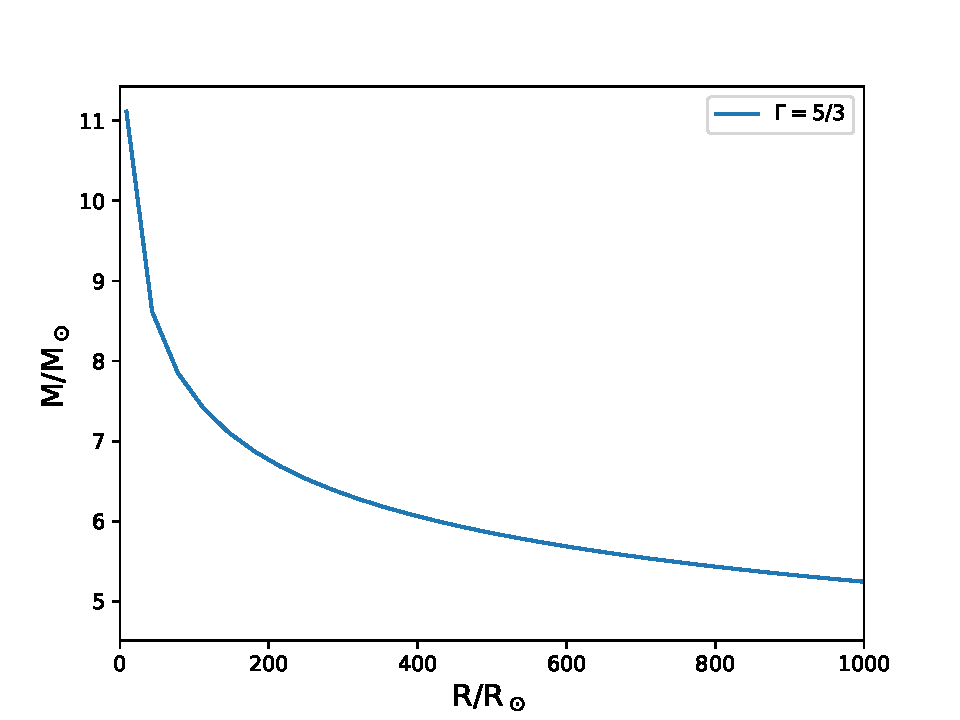
\includegraphics[width=0.7\textwidth, angle=0]{images/polytrope_own.pdf}
%\captionsetup{width=.8\textwidth}
%\caption{Mass-radius relation for a non-relativistic polytropic star}
%\caption*{This mass-radius diagram was computed from equation \ref{M-R}, for a polytropic star with $k=10^{15}$, $\Gamma=5/3$ and a central desity $\rho_0=10^{12}$}. 
%\label{polytropes1}
%\end{center}
%\end{figure}
%
%\FloatBarrier






\newpage

%\section{General relativity}
%
%The need for a complete theory of gravity became apparent in the 19th century. Astronomical observations yielded data that violated the predictions of Newtonian gravity, among them mercury's perihelion shift\cite{1859AnPar...5....1L}, light deflection by the sun \cite{1920RSPTA.220..291D}, gravitational redshift in Sirius B \cite{2010JHA....41...41H}, and others. So far, Einstein's general relativity(GR) has proven accurate in describing these phenomena. In particular, as far as this research is concerned, it describes well the evolution and structure of the most compact objects in the universe: black holes, neutron stars, and binary systems that contain them.
%
%GR has predicted that binary systems of compact objects lose radial separation due to significant emission of gravitational radiation. Such effects have been frequently observed in BNS systems by Hulse and Taylor \cite{Weisberg:1981mt} and LIGO\cite{LIGOScientific:2017vwq}, BBH by LIGO and Virgo \cite{LIGOScientific:2016aoc}, and NSBH by LIGO Virgo and KAGRA\cite{LIGOScientific:2021qlt}. Unfortunately, the two-body problem in GR has no analytical solution. Such systems and their gravitational waves must be studied by approximate and semi-analytical methods in their premerger stage or by numerical methods if one intends to study the complete evolution of the inspiral-merger-postmerger system\cite{Dietrich:2018phi}.
%
%Although Einstein's general relativity is a broad theory with relevant consequences in several areas of astrophysics, the following section intends to make a simple introduction to the field equations, motivated by several sources such as the books by Inverno\cite{inverno}, Wald\cite{Wald:1984rg}, and Carroll\cite{carroll-notes}. Later it develops in a detailed way relativistic aspects of the physics of stars in hydrostatic equilibrium and gravitational waves, following in general lines, what is presented in the books of Weinberg\cite{Weinberg:1972kfs} and Hartle\cite{Hartle:2021pel}. Other solutions to the field equations and details on differential geometry and topology are briefly mentioned but not developed.
%
%
%
%\subsection{Einstein's field equations}
%
%After revolutionizing physics with the theory of special relativity in 1905 \cite{Einstein:1905}, Einstein took a few more years to elaborate a more general theory that could intrinsically include gravity in spacetime's geometry \cite{Einstein:1915ca}.
%
%Various physical ideas and principles led Einstein to derive his field equations. In particular, Mach's principle \cite{mach1919science, 1995mpfn.conf.....B} and the equivalence principle largely influenced his theory. The geometry of spacetime, being responsible for the inertial motion of bodies and the mass/energy distribution of the universe contributing to that inertia, led Einstein to a set of tensor field equations relating the spacetime metric and its derivatives to the energy-momentum tensor of matter and fields living in it. However, other methods have been used to obtain the field equations, such as Hilbert \cite{Hilbert:1915tx} and Lovelock \cite{Lovelock:1971yv}. 
%
%In 3+1 dimensions, they are a set of 10 independent, second-order, coupled, nonlinear partial differential equations over the spacetime metric $g_{\mu \nu}$, that can be written in two compact forms
%
%
%
%\begin{equation}\label{EFE}
%G_{\mu\nu}  =  \frac{8\pi G}{c^4} \cdot T_{\mu\nu},
%\end{equation}
%
%\begin{equation}\label{EFE-ricci}
%R_{\mu\nu}  =  \frac{8\pi G}{c^4} \cdot (T_{\mu\nu} - \frac{1}{2} g_{\mu\nu} T), 
%\end{equation}
%
%Where G and c are the gravitational constant and the speed of light in vaccuum. $R_{\mu\nu}$, $R$ and $G_{\mu\nu}$ are called Ricci tensor, Ricci scalar and Einstein tensor respectively, and their definitions are listed below, to help unveil that equations \ref{EFE} and \ref{EFE-ricci} are in fact, partial diferential equations for the metric components $g_{\mu\nu}$.
%
%
%\begin{itemize}
%\item Christoffel symbols
%
%\begin{equation}\label{christoffel}
%\Gamma^{\alpha}_{\beta \gamma} = \frac{1}{2} g^{\alpha \delta}(\partial_{\beta} g_{\delta \gamma} + \partial_{\gamma} g_{\delta \beta} - \partial_{\delta} g_{\beta \gamma})
%\end{equation}
%
%\begin{equation}
%\Gamma^{\alpha}_{\beta \gamma} = \Gamma^{\alpha}_{\gamma \beta}
%\end{equation}
%
%
%\item The Riemann tensor, Ricci tensor and Ricci scalar 
%\begin{equation}
%R^{\alpha}_{\mu\gamma \delta} = \partial_{\gamma} \Gamma^{\alpha}_{\mu \delta} - \partial_{\delta} \Gamma^{\alpha}_{\gamma \mu} +  \Gamma^{\alpha}_{\gamma \lambda} \Gamma^{\lambda}_{\delta \mu} - \Gamma^{\alpha}_{\delta \lambda} \Gamma^{\lambda}_{\gamma \mu}
%\end{equation}
%
%\begin{equation}
%R_{\alpha \beta}= R^{\delta}_{\alpha \delta \beta}
%\end{equation}
%
%\begin{equation}
%R = g^{\alpha \beta}R_{\alpha \beta}
%\end{equation}
%
%\item The Einstein tensor, i.e. the trace reversed Ricci tensor
%
%\begin{equation}
%G_{\mu\nu} = R_{\mu\nu} - \frac{1}{2} g_{\mu\nu} R
%\end{equation}
%
%
%\end{itemize}
%
%
%Obtaning the spacetime metrics and solving the geodesic equations 
%
%\begin{equation}\label{par-trans}
%u^{\delta} \nabla_{\delta } u^{\alpha } = 
%0 \rightarrow \frac{d^2 x^{\alpha}}{d\tau^2} = - \Gamma^{\alpha}_{\nu\mu} \frac{dx^{\nu}}{d\tau} \frac{dx^{\mu}}{d\tau}
%\end{equation}
%
%Is the relativistic analogous to what in newtonian case would require solving the Poisson equation \ref{poisson} and obtaining particle trayectories on the gravitational field using Newton's second law. Where  $\nabla_{\delta}$ are the components of the covariant derivative operator acting on the particle's 4-velocity $u^{\alpha}$. In addition, tidal interactions can be measured by the geodesic deviation equation(see Hartle \cite{Hartle:2021pel} section 7)
%
%\begin{equation}\label{tidal1}
%\frac{d \xi^{\alpha}}{d\tau} = - R^{\alpha}_{\;\; \tau \mu \tau} \cdot \xi^{\mu}
%\end{equation} 
%
%Which looks similar to its newtonian analogous as well, but involves the geometry of spacetime via the Riemann tensor components $R^{\alpha}_{\;\; \tau \mu \tau}$.
%
%On the other hand, the right hand side of the equations contains information about the fluids, particles and fields present in spacetime. However, defining quantities such as mass-energy in a global way in a curved spacetime is more complicated than in the flat Minkowski spacetime used in special relativity. Spacetime and stress-energy are coupled, such that physically relevant solutions to the field equations must satisfy $\nabla_{\mu} T^{\mu\nu} = 0$, since the second bianchi identity leads to zero divergence of the einstein tensor $\nabla_{\mu}G^{\mu\nu} = 0$ (see \cite{inverno, Wald:1984rg, Weinberg:1972kfs}.
%
%Some energy-momentum tensors have been inherited from special relativity and have given rise to analytical solutions of the einstein equations such as the TOV equation \cite{PhysRev.55.374} and the Reinser-Nordstrom solution \cite{https://doi.org/10.1002/andp.19163550905}. In a local inertial frame, the stress-energy tensor for perfect fluids, and the Faraday tensor can be written as
%
%
%\begin{equation}
%T^{\mu \nu} = 
%\begin{pmatrix}
%\rho \cdot c^2&0&0&0 \\
%0&-p&0&0 \\
%0&0&-p&0 \\
%0&0&0&-p\\
%\end{pmatrix} \;\; ,
%\end{equation}
%
%\begin{equation}
%F_{\mu \nu} = 
%\begin{pmatrix}
%0&\frac{E_x}{c}&\frac{E_y}{c}&\frac{E_z}{c} \\
%-\frac{E_x}{c} &0   &B_z  &B_y \\
%-\frac{E_y}{c} &-B_z&0    &B_x \\
%-\frac{E_z}{c} &-B_y&-B_x &0\\
%\end{pmatrix} \;\;,
%\end{equation}
%
%
%Where $\rho$ is the rest mass density, p is the pressure, $E_i$ is the ith component od the electric field, $B_j$ is the jth component of a magnetic field and c is the speed of ligth in vaccum. Both have been relevant in theoretical applications of GR like idealized neutron stars or quark-gluon plasmas \cite{Nagle_2011}, and charged black holes respectively \cite{PhysRevD.13.2713}.
%
%Due to their nonlinear and coupled character, analytical solutions to the Einstein equations are challenging to find. This is why approximate methods such as post-Newtonian expansions and numerical solutions have been frequently used in the last decades. Although this thesis deals with gravitational waves extracted from fully relativistic numerical simulations, a detailed development of the first-order approximation used by Einstein in 1916 and of the Tolman-Oppenheimer-Volkoff equation follows. 
%
%The existence of gravitational waves and their predominantly quadrupole nature are fundamental in constructing waveform models for compact binary mergers, as well as the existence of a maximum mass for a static star given an equation of state to understand the gravitational collapse of neutron star postmerger remnants.
%
%
%
%
%\subsection{Spherically symmetric stars and the TOV equation}
%
%Currently, General relativity is the best tool we have to study the physics of compact objects like Neutron stars and black holes. Newtonian physics does not represent a good model since their gravitational fields are powerful and can not be studied in the Newtonian approximation(see table \ref{compactness}). Their internal structure can be studied using a generalized version of equation \ref{press.grad} called the Tolmann-Oppenheimer-Volkoff equation, which, together with the matter model encoded in an equation of state, will tell about the internal structure of a spherically symmetric star via its pressure and density profiles. Mass-radius diagrams have been widely used in the literature for stiffer and softer equations of state to see whether they support a maximum mass within the current experimental bounds known from pulsars and gravitational wave events like GW170817.
%
%Let us start with a static and spherically symmetric spacetime metric of the form \ref{metric} in geometric units (see appendix \ref{unit conv})
%
%\begin{equation}\label{metric}
%ds = B(r) dt \otimes dt - A(r) dr \otimes dr - r^2 (d\theta^2 + \sin^2 \theta \; d\phi^2)
%\end{equation}
%
%Its non-vanishing Ricci tensor components \cite{Weinberg:1972kfs} can be given in terms of the functions $A(r)$ and $B(r)$.
%
%\begin{equation}\label{E1}
%R_{rr} = \frac{B''}{2B} - \frac{B'}{4B} \left( \frac{A'}{A}+\frac{B'}{B} \right) - \frac{A'}{rA} = -4\pi G(\rho-P) A
%\end{equation}
%
%\begin{equation}\label{E2}
%R_{\theta \theta}  = -1 + \frac{r}{2A} \left( -\frac{A'}{A} + \frac{B'}{B} \right) + \frac{1}{A} = -4\pi G(\rho - P) r^2
%\end{equation}
%
%\begin{equation}\label{E3}
%R_{tt} = - \frac{B''}{2A} + \frac{B'}{4A} \left( \frac{A'}{A}+\frac{B'}{B} \right) - \frac{B'}{rA} = - 4\pi G (\rho + 3P) B
%\end{equation}
%
%Let us consider the Energy momentum tensor of a perfect fluid given by 
%
%\begin{equation}
%T^{\mu \nu} = (\rho + P) u^\mu u^\nu + P g^{\mu \nu}
%\end{equation}
%
%The energy-momentum conservation can be used to obtain an expression for the metric coefficient $B(r)$
%\begin{equation}
%0 = \nabla_\nu T^{\mu \nu} = \partial_\nu T^{\mu \nu} + \gamma^\mu_{\nu \delta} T^{\delta \nu} + \gamma^\nu_{\nu \delta} T^{\mu \delta}
%\end{equation}
%
%\begin{equation}
%\begin{matrix}
%0 = (\partial_\nu P) g^{\mu \nu} + P \partial_\nu g^{\mu \nu} +\partial_\nu \left[ (P+\rho) u^\mu u^\nu \right]+ \\ \Gamma^\nu_{\nu \delta}(P g^{\mu \delta} + (\rho+P)u^\mu u^\delta ) + P \Gamma^\mu_{\nu \delta} g^{\nu \delta} +\Gamma^\mu_{\nu \delta} (\rho+ P) u^\delta u^\nu.
%\end{matrix}
%\end{equation}
%
%\begin{equation}
%0 = (\partial_\nu P) g^{\mu \nu} + \Gamma^\nu_{\nu \delta}(P g^{\mu \delta} + (\rho+P)u^\mu u^\delta ) + \partial_\nu \left[ (P+\rho) u^\mu u^\nu \right]+ \Gamma^\mu_{\nu \delta} (\rho+ P) u^\delta u^\nu.
%\end{equation}
%
%\begin{equation}\label{per-flu}
%\begin{matrix}
%0 = (\partial_\nu P) g^{\mu \nu} + g^{-\frac{1}{2}}\partial_\nu(g^{\frac{1}{2}})  (P g^{\mu \delta} + (\rho+P)u^\mu u^\delta ) + \partial_\nu \left[ (P+\rho) u^\mu u^\nu \right]+ \Gamma^\mu_{\nu \delta} (\rho+ P) u^\delta u^\nu.
%\end{matrix}
%\end{equation}
%
%where we have used the identity $\Gamma^\mu_{\mu \nu}=g^{-\frac{1}{2}}\partial_\nu(g^{\frac{1}{2}})$(see \cite[section 7]{inverno}) and the compatibility of the metric to eliminate some terms. Further, we evaluate energy-momentum conservation in the rest frame of the fluid, where its 4-velocity takes the form $u=(\sqrt{g_{00}},0,0,0,0)$.  In such a frame, equation \ref{per-flu} takes a much simpler form since only the timelike components of the 4-velocity contribute, and the pressure and density profiles will not depend on time. The relevant Christoffel symbols also take a simple form, and the metric trace vanishes after differentiation. 
%
%\begin{equation}
%0 = (\partial_\nu P) g^{\mu \nu} + \Gamma^\mu_{00} (\rho+ P) (u^0)^2 + \partial_0 \left[ (P+\rho) u^\mu u^0 \right]
%\end{equation}
%
%\begin{equation}
%0 = (\partial_\nu P) g^{\mu \nu} + \left(-\frac{1}{2}g^{\mu \nu} \partial_\nu g_{00} \right) (\rho+ P) (u^0)^2 
%\end{equation}
%
%\begin{equation}
%-(\partial_\nu P) g^{\mu \nu} = (\rho+ P) g^{\mu \nu} \partial_\nu \ln{(-g_{00})^{\frac{1}{2}}}
%\end{equation}
%
%\begin{equation}\label{ener.cond0}
%-\partial_\lambda P  = (\rho+ P)  \partial_\lambda \ln{(-g_{00})^{\frac{1}{2}}}
%\end{equation}
%
%Taking $g_{00} = -B(r)$, equation \ref{ener.cond0} becomes an equation for B and its first derivative
%
%\begin{equation}\label{B'/B}
%\frac{-2P'}{(P+\rho)} = \frac{B'}{B}
%\end{equation}
%
%
%To get an equation for $A$ and $\frac{A'}{A}$, we use the following combination of the Ricci tensor components.
%
%\begin{equation}
%\frac{R_{rr}}{2A} +\frac{R_{\theta \theta}}{r^2} + \frac{R_tt}{2B} = -\frac{A'}{rA^2} - \frac{1}{r^2} + \frac{1}{A r^2} = -8\pi G \rho
%\end{equation}
%
%\begin{equation}
%\frac{1}{r^2} \left[ \left(\frac{r}{A} \right)' - 1 \right] = -8\pi G \rho
%\end{equation}
%
%\begin{equation}
% \left(\frac{r}{A}\right)' = 1 - 8\pi G r^2 \rho
%\end{equation}
%
%\begin{equation}
%\left(\frac{r}{A}\right) = r - 2G \int_0^r dr'4\pi  r'^2 \rho(r')
%\end{equation}
%
%\begin{equation}
%\left(\frac{r}{A}\right) = r - 2G M(r) \rightarrow M(r):= \int_0^r dr'4\pi  r'^2 \rho(r')
%\end{equation}
%
%\begin{equation}\label{A}
%A = \left[ 1 - \frac{2G M(r)}{r} \right]^{-1} \rightarrow M(r):= \int_0^r dr'4\pi  r'^2 \rho(r')
%\end{equation}
%
%\begin{equation}\label{A'/A}
%\frac{A'}{A} = \frac{2G(M/r)'}{1-\frac{2GM(r)}{r}}
%\end{equation}
%
%
%Finally one can insert equations \ref{A},\ref{A'/A} and \ref{B'/B}, in  $R_{\theta \theta}$ to get an equation for the pressure gradient in terms of $M(r)$, $P(r)$ and $\rho(r)$: The TOV equation.
%
%\begin{equation}
%-1 + \frac{r}{2A} \left( -\frac{A'}{A} + \frac{B'}{B} \right) + \frac{1}{A} = -4\pi G(\rho - P) r^2
%\end{equation}
%
%\begin{equation}
%-1 + Gr \left( \frac{M}{r}\right)' - \left[ 1-\frac{rP'}{(P+\rho)} \right] = -4\pi G(\rho - P) r^2
%\end{equation}
%
%\begin{equation}
%-1 + \frac{GM}{r^2} -\frac{GrM'}{r} - \left[ 1-\frac{rP'}{(P+\rho)} \right] = -4\pi G(\rho - P) r^2
%\end{equation}
%
%\begin{equation}
%-GM' - \left[ 1 - \frac{2GM}{r}\right] - \left[ 1-\frac{rP'}{(P+\rho)} \right]\left(  1 - \frac{2GM}{r} \right) = -4\pi G(\rho - P) r^2
%\end{equation}
%
%\begin{equation}
%-1 + \left[ 1-\frac{rP'}{(P+\rho)} \right]\left(  1 - \frac{2GM}{r} \right)+\frac{GM}{r} - 4\pi G r^2 \rho(r) = -4\pi G(\rho - P) r^2
%\end{equation}
%
%\begin{equation}
%-1 + \left[ 1-\frac{rP'}{(P+\rho)} \right]\left(  1 - \frac{2GM}{r} \right)+\frac{GM}{r} - 4\pi G r^2 \rho(r) = -4\pi G(\rho - P) r^2
%\end{equation}
%
%\begin{equation}
%- \left( \frac{rP'}{(P+\rho)}\right)\left(  1 - \frac{2GM}{r} \right) - \frac{GM}{r} = + 4\pi G P r^2
%\end{equation}
%
%\begin{equation}
%- \left( \frac{rP'}{(P+\rho)}\right)\left(  1 - \frac{2GM}{r} \right) = \frac{G}{r} \left( M + 4\pi r^3 P \right)
%\end{equation}
%
%\begin{equation}
%- \left( \frac{P'}{(P+\rho)}\right) = \frac{G}{r^2} \frac{\left( M + 4\pi r^3 P \right)}{\left(  1 - \frac{2GM}{r} \right)}
%\end{equation}
%
%\begin{equation}
%- P' = \frac{G}{r^2} \frac{\left( M + 4\pi r^3 P \right)}{\left(  1 - \frac{2GM}{r} \right)} (P+\rho)
%\end{equation}
%
%\begin{equation}\label{TOV2}
%- P' = \frac{G}{r^2} \frac{\left( M + 4\pi r^3 \frac{P}{c^2} \right)}{\left(  1 - \frac{2GM}{r c^2} \right)} (\frac{P}{c^2}+\rho)
%\end{equation}
%
%Notice how equation \ref{TOV2} reduces to the Newtonian structure equation \ref{press.grad} when taking the limits $c\rightarrow \infty$ and $GM/c^2 <<1$. The relativistic more general equation is much more complicated than its Newtonian counterpart and does not allow a simple analytic treatment for the polytropic equations of state. Figure \ref{equations of state and tidal deformability} shows several examples of EOSs available in the literature, which are usually presented by the mass-radius diagram resulting from solving the TOV equation numerically. One of the most important features is the maximum of each curve, called the maximum TOV mass, and serves as a reference of how heavy can a compact object be for the given equation of state. Scientists have investigated the existence of a threshold mass parametrized by the ratio of its total gravitational mass and the maximum TOV mass.
%
%\begin{equation}\label{delta}
%\delta=\frac{M_g}{M_{TOV}}
%\end{equation} 
%
%
%\begin{figure}[hbt!]
%\begin{center}
%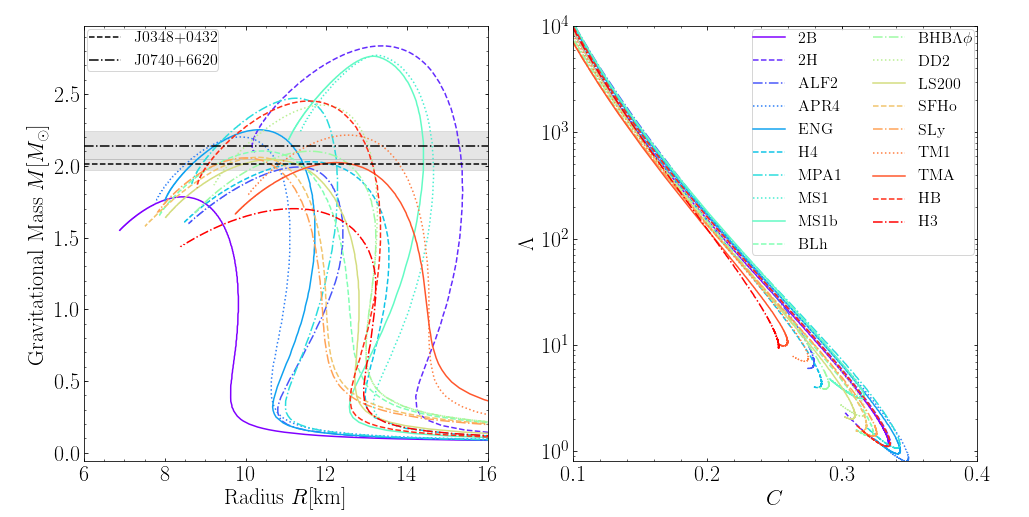
\includegraphics[width=\textwidth, angle=0]{images/EOS_TOV.png}
%\caption{Equation of state database used in the CoRe catalog \cite{Dietrich:2018phi}}
%\label{equations of state and tidal deformability}
%\end{center}
%This image was taken from \cite{EOSDB}. It shows the mass-radius relations for some equations of state in the database(left) and their tidal deformability-compactness relation(right). 
%\end{figure}
%
%\FloatBarrier
%
%
%
%\subsection{Linearized theory and gravitational radiation}\label{GW}
%
%Einstein did not take too long to come up with the first approximate solution of his equations in 1916 \cite{Einstein:1916cc}. He computed it by expanding the metric $g$ to first order, around the background Minkowski metric. 
%
%\begin{equation}
%g_{_{\mu \nu}} =  \eta_{_{\mu \nu}} + h_{_{\mu \nu}}.
%\end{equation}
%
%Where the components of $h_{_{\mu \nu}}$ are said to be a small, i.e. $h_{_{\mu \nu}}<<1$ as compared to Minkowski metric $\eta_{_{\mu \nu}}$  in an affine chart $x^\mu$ where its components are $diag(-1,1,1,1)$. Such first-order approximation will allow the Christoffel symbols to be written in terms of the metric perturbation and its derivatives
%
%\begin{equation}
%\Gamma^{^{\alpha}}_{_{\beta \gamma}} = \frac{1}{2} \eta^{^{\alpha \delta}}(\partial_{_{\beta}} h_{_{\delta \gamma}} + \partial_{_{\gamma}} h_{_{\delta \beta}} - \partial_{_{\delta}} h_{_{\beta \gamma}}),
%\end{equation}
%
%The Riemann tensor, the Ricci tensor, and the Ricci scalar have a much simpler form in a coordinate chart $x^\mu$.
%
%\begin{equation}
%R^{^{\alpha}}_{_{\beta \mu\nu}} = -\frac{1}{2} \eta^{^{\alpha \lambda}} [ \partial^2_{_{\lambda \mu}} h_{\beta \nu} + \partial^2_{_{\beta \nu}} h_{\lambda \mu} - \partial^2_{_{\lambda \nu}} h_{\beta \mu} - \partial^2_{_{\beta \mu}} h_{\lambda \nu}],
%\end{equation}
%
%\begin{equation}
%R_{_{\beta \nu}} = -\frac{1}{2} [ \Box h_{\beta \nu} + \partial_{_{\beta}}\partial_{_{\nu}} h - \partial_{_{\nu}} \partial^{^{\gamma}} h_{_{\beta \gamma}} - \partial_{_{\beta}} \partial^{^{\lambda}} h_{_{\lambda \nu}} ],
%\end{equation}
%
%\begin{equation}
%R_{_{\beta \nu}} = -\frac{1}{2} [ \Box h_{\beta \nu} + \partial_{_{\beta}}\partial_{_{\nu}} h - \partial_{_{\nu}} \partial^{^{\gamma}} h_{_{\beta \gamma}} - \partial_{_{\beta}} \partial^{^{\lambda}} h_{_{\lambda \nu}} ],
%\end{equation}
%
%
%\begin{equation}
%R = -\frac{1}{2} \Box h + \partial^{^{\alpha}}\partial^{^{\beta}} h_{_{\alpha \beta}}.
%\end{equation}
%
%Motivated by equation \ref{EFE1},  where the Einstein tensor is used to make the equations look more compact, one can also use a reversed version of $h$, namely $\bar{h}_{_{\mu\nu}} = h_{_{\mu\nu}}-\frac{1}{2} \eta_{_{\mu\nu}} h$  
%
%\begin{equation}
%R_{_{\beta \nu}} = -\frac{1}{2} [ \Box( \bar{h}_{_{\beta \nu}}-\frac{1}{2} \eta{_{\beta \nu}} \bar{h} ) + - \partial_{_{\nu}} \partial^{^{\gamma}} \bar{h}_{_{\beta \gamma}} - \partial_{_{\beta}} \partial^{^{\lambda}} \bar{h}_{_{\lambda \nu}} ]
%\end{equation}
%
%\begin{equation}
%R = -\frac{1}{2} \Box \bar{h} + \partial^{^{\alpha}}\partial^{^{\beta}} \bar{h}_{_{\alpha \beta}}
%\end{equation}
%
%
%Then, to first order equations \ref{EFE1} and \ref{EFE2} become second order partial differential equations in $h_{_{\mu\nu}}$ and $\bar{h}_{_{\mu \nu}}$  
%
%\begin{equation}\label{hbar}
%G^{(1)}_{_{\mu\nu}} = \frac{8\pi G}{c^4} T^{(1)}_{_{\mu\nu}} \rightarrow \bar{\mathcal{D}}^{^{\mu\nu}}_{_{\alpha \beta}} \bar{h}_{_{\mu\nu}} = \frac{8\pi G}{c^4} T^{(1)}_{_{\mu\nu}}
%\end{equation}
%
%
%\begin{equation}\label{h}
%R^{(1)}_{_{\mu\nu}} = \frac{8\pi G}{c^4}(T^{(1)}_{_{\mu\nu}} - \frac{1}{2} \eta_{_{\mu\nu}}T^{(1)}) \rightarrow \mathcal{D}^{^{\mu\nu}}_{_{\alpha \beta}} h_{_{\mu\nu}} = \frac{8\pi G}{c^4}(T^{(1)}_{_{\mu\nu}} - \frac{1}{2} \eta_{_{\mu\nu}}T^{(1)})
%\end{equation}
%
%
%Where $\mathcal{D}$ and $\mathcal{\bar{D}}$ are second order differential operators.
%
%\begin{equation}
%\mathcal{D}^{^{\mu\nu}}_{_{\alpha \beta}} = -\frac{1}{2}( \delta^{^{\mu}}_{_{\alpha}} \delta^{^{\nu}}_{_{\beta}} \Box + \eta^{^{\mu\nu}}\partial_{_{\alpha}}\partial_{_{\beta}} - \delta^{^{\nu}}_{_{\beta}} \partial_{_{\alpha}}\partial^{^{\mu}} - \delta^{^{\nu}}_{_{\alpha}} \partial_{_{\beta}}\partial^{^{\mu}}),
%\end{equation}
%
%\begin{equation}
%\bar{\mathcal{D}}^{^{\mu\nu}}_{_{\alpha \beta}} = -\frac{1}{2}( \delta^{^{\mu}}_{_{\alpha}} \delta^{^{\nu}}_{_{\beta}} \Box + \eta^{^{\alpha \beta}}\partial^{^{\mu}}\partial_{_{\nu}} - \delta^{^{\nu}}_{_{\beta}} \partial_{_{\alpha}}\partial^{^{\mu}} - \delta^{^{\nu}}_{_{\alpha}} \partial_{_{\beta}}\partial^{^{\mu}}).
%\end{equation}
%
%
%Equations \ref{h} and \ref{hbar} will determine the space-time perturbations $h$ or $\bar{h}$ up to redefinitions of the form $h^{'}_{_{\mu\nu}}$ and $\bar{h}^{'}_{_{\mu\nu}}$ due to the gauge freedom of general relativity comming from infinitesimal isometries of space-time \cite{Wald:1984rg}.
%
%\begin{equation}
%h_{_{\mu\nu}} \rightarrow  h^{'}_{_{\mu\nu}} = h_{_{\mu\nu}} + \partial_{\mu} \Lambda_{_{\nu}} + \partial_{\nu} \Lambda_{_{\mu}} 
%\end{equation}
%
%
%\begin{equation}
%\bar{h}_{_{\mu\nu}} \rightarrow  \bar{h}^{'}_{_{\mu\nu}} = \bar{h}_{_{\mu\nu}} + \partial_{_{\mu}} \Lambda_{_{\nu}} + \partial_{_{\nu}} \Lambda_{_{\mu}} - \eta_{_{\mu\nu}} \partial^{^{\delta}} \Lambda_{_{\delta}}
%\end{equation}
%
%Gauge fixing can be performed in several ways; however, the de Donder gauge fixing is the most common one and allows us to determine the $\Lambda$s using retarded greens functions. However, solutions to $\Box \Lambda_\nu = 0$ can also be added.
%
%\begin{equation}
%\partial^{^{\mu}} \bar{h}^{'}_{_{\mu\nu}} = 0
%\end{equation}
%
%
%\begin{equation}
%\partial^{^{\mu}}\bar{h}_{_{\mu\nu}} + \partial^{^{\mu}}\partial_{_{\mu}} \Lambda_{_{\nu}} + \partial^{^{\mu}}\partial_{_{\nu}} \Lambda_{_{\mu}} - \partial^{^{\mu}}(\eta_{_{\mu\nu}} \partial^{^{\delta}} \Lambda_{_{\delta}}) = 0
%\end{equation}
%
%
%\begin{equation}
%\partial^{^{\mu}}\bar{h}_{_{\mu\nu}} + \Box\Lambda_{_{\nu}} = 0 \;\;\;, \Box \Lambda_\nu = 0
%\end{equation}
%
%\begin{equation}\label{dedonder0}
%\partial^{^{\mu}}\bar{h}_{_{\mu\nu}} = 0
%\end{equation}
%
%
%and inserting \ref{dedonder0} in equation \ref{hbar}, the first order Einstein's field equations become simple wave equations for $\bar{h}_{_{\mu\nu}}$ with a source $T^{(1)}_{_{\mu\nu}}$
%
%
%\begin{equation}
%\left( -\frac{1}{2} \delta^{^{\mu}}_{_{\alpha}} \delta^{^{\nu}}_{_{\beta}} \Box \right) \bar{h}_{_{\mu\nu}} = \frac{8\pi G}{c^4} T^{(1)}_{_{\mu\nu}}
%\end{equation}
%
%
%\begin{equation}\label{dedonder1}
%\Box\bar{h}_{_{\mu\nu}} = -\frac{16\pi G}{c^4} T^{(1)}_{_{\mu\nu}},
%\end{equation}
% 
%
%Finally, both equations \ref{dedonder0} and \ref{dedonder1} must be satisfied simultaneously, and the metric perturbations can be computed using retarded Green's functions in the non-vacuum case. i.e. $T^{(1)}_{_{\mu\nu}} \neq 0$ and form a pair that completely determines the system of equations \ref{EFE1} to first order 
%
%\begin{equation}\label{lin.efe0}
%\begin{cases}
%\Box  \bar{h}_{_{\mu\nu}} = \frac{16\pi G}{c^4} T^{(1)}_{_{\mu\nu}} \rightarrow \bar{h}_{_{\mu\nu}}(\vec{x}) = -\frac{16\pi G}{c^4} \left( \frac{1}{4\pi} \int d^3x' \frac{T_{_{\mu\nu}} \left( t - \frac{|| \vec{x}-\vec{x}' ||}{c} , \vec{x}' \right)  }{|| \vec{x}-\vec{x}' ||} \right)\\
%\partial^{^{\mu}} \bar{h}_{_{\mu\nu}} = 0 
%\end{cases}
%\end{equation}
%
%
%\subsection{Transverse traceless gauge}
%
%In contrast to Newtonian gravity, solutions to the vacuum field equations are already interesting enough to be studied since the d'Alembert operator allows wave-like solutions.  The simplest Anzats one can think of is a plane wave solution of the form 
%
%\begin{equation}
%h_{_{\mu\nu}} = A_{_{\mu\nu}} e^{i k_{_{\delta}} \cdot x^{{\delta}}},
%\end{equation}
%
%where $k = (w, \vec{k})$ being a lightlike vector, i.e. $k^{^{\delta}}k_{_{\delta}} = 0$  gives the dispersion relation for gravitational waves
%
%\begin{equation}
%-w^2 + || \vec{k} || = 0
%\end{equation}
%
%It can be shown that adding the following conditions, also called Transverse traceless gauge, on top of the De Donder gauge closes the remaining gauge freedom completely.
%
%\begin{equation}
%h_{_{0i}} = 0  \hspace{1cm} h_{_{00}} = 0
%\end{equation} 
%
%
%\begin{equation}
%h^{^{\delta}}_{_{\delta}} = 0  \hspace{1cm} k^{i}h_{_{ij}} = 0
%\end{equation}
%
%There are only two independent components out of the initial 10. The tensor components $h_{_{\mu\nu}}$ can be written in terms of the  polarizations $h_+$ and $h_\times$. 
%
%\begin{itemize}
%\item for a wave propagating in the z-direction.
%
%\begin{equation}
%h_{\mu \nu} \theta^\mu \otimes \theta^\nu = 
%\begin{pmatrix}
%0&0&0&0 \\
%0&h_+ &h_\times &0 \\
%0&h_\times &-h_+ &0 \\
%0&0&0&0 \\
%\end{pmatrix} 
%\end{equation}
%
%So the line element $ds = (\eta_{_{\mu \nu}} + h_{_{\mu \nu}}) dx^\mu \otimes dx^\nu $ would become:
%
%\begin{equation}\label{GWlineelement}
%ds^2 = c^2 dt \otimes dt - (1-h_+) dx \otimes dx - (1+h_+) dy \otimes dy + h_\times dx \otimes dy + h_\times dy \otimes dx
%\end{equation}
%
%\item for a wave propagating in the x-direction
%
%\begin{equation}
%h_{\mu \nu} \theta^\mu \otimes \theta^\nu = 
%\begin{pmatrix}
%0&0&0&0 \\
%0&0&0&0 \\
%0&0&h_+& h_\times \\
%0&0&h_\times& - h_+\\
%\end{pmatrix}
%\end{equation}
%
%\begin{equation}
%ds^2 =  c^2 dt \otimes dt - (1+h_+) dy \otimes dy - (1-h_+) dz \otimes dz + h_{\times} dy \otimes dz + h_{\times} dz \otimes dy
%\end{equation}
%
%
%\item for a wave propagating in the y-direction
%\begin{equation}
%h_{\mu \nu} \theta^\mu \otimes \theta^\nu = 
%\begin{pmatrix}
%0&0&0&0 \\
%0&h_+&0&h_\times \\
%0&0&0&0 \\
%0&h_\times&0&-h_+ \\
%\end{pmatrix} 
%\end{equation}
%
%\begin{equation}
%ds^2 =  c^2 dt \otimes dt - (1+h_+) dx \otimes dx - (1-h_+) dz \otimes dz + h_{\times} dx \otimes dz + h_{\times} dz \otimes dx
%\end{equation}
%
%\end{itemize}
%
%
%Effects of gravitational waves can be measured by using the geodesic deviation equation \ref{tidal2}, which is the generalization of equation X. Which can be translated into tidal accelerations between test masses, or proper length changes in their relative distances \cite{Hartle:2021pel, carroll-notes}
%
%\begin{equation}\label{tidal2}
%\frac{d^2 \xi^{\mu}}{d\tau^2} = R^{\mu}_{\hspace{1mm} \tau \nu \tau} \xi^{\nu}
%\end{equation}
%
%
%For example,  two test masses moving along geodesics separated by $\xi$ in the x direction, i.e. $\xi^\mu = (0,\xi,0,0)$ will experience a a tidal acceleration in the x and y direction if there is an incoming gravitational wave in the z direction:
%
%\begin{equation}
%\frac{d^2 \xi^{\mu}}{d\tau^2} = \frac{1}{2}\xi \frac{d^2 h_+}{d\tau^2} \hspace{10mm} \frac{d^2 \xi^{\mu}}{d\tau^2} = \frac{1}{2}\xi \frac{d^2 h_\times}{d\tau^2}
%\end{equation}
%
%
%And for two geodesics separated by $\xi$ in the y direction, i.e., $\xi^\mu = (0,0,\xi,0)$ the tidal acceleration in the x and y direction is given by:
%
%\begin{equation}
%\frac{d^2 \xi^{\mu}}{d\tau^2} = \frac{1}{2}\xi \frac{d^2 h_\times}{d\tau^2},\hspace{10mm} \frac{d^2 \xi^{\mu}}{d\tau^2} = -\frac{1}{2}\xi \frac{d^2 h_+}{d\tau^2}
%\end{equation}
%
%
%\begin{figure}[hbt!]
%\begin{center}
%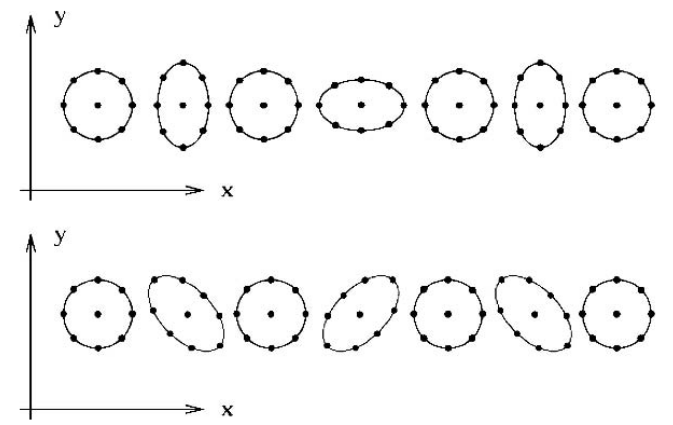
\includegraphics[width=0.6\textwidth, angle=0]{images/particle-ring.png}
%\caption{Tidal forces on a ring of test masses}
%\label{GW passing through a ring of test masses}
%\end{center}
%This image was taken from \cite{carroll-notes}.  it shows The effects of the $h_+$ (top) and $h_\times$ polarizations of gravitational waves on a ring of test masses.The phases shown are 0, $\frac{\pi}{2}$, $\pi$, $\frac{3\pi}{2}$, and $2\pi$ respectively.
%\end{figure}
%
%\FloatBarrier
%
%
%
%\subsection{Gravitational wave generation}
%
%Finding metric perturbations through equations \ref{pert.int} can be done analytically for a few cases. It will be further shown that only sources with time-varying quadrupole moment \ref{quadrupole} will generate gravitational radiation. Examples of them can be binary systems \cite{Hartle:2021pel} and deformed rotating stars \cite{Creighton:2011zz}.
%
%\begin{equation}\label{pert.int}
%\bar{h}_{_{uv}}(\vec{x}) = -\frac{16\pi G}{c^4} \left( \frac{1}{4\pi} \int d^3x' \frac{T_{_{uv}} \left( t - \frac{|| \vec{x}-\vec{x}' ||}{c} , \vec{x}' \right)  }{|| \vec{x}-\vec{x}' ||} \right)
%\end{equation}
%
%
%Let us start by rewriting the spatial components of the energy-momentum tensor using the following identities.
%
%\begin{equation}
%T^{ij} = \frac{1}{2} [\delta^{i}_{m} \delta^{j}_{l} + \delta^{i}_{l} \delta^{j}_{m}] T^{lm} = \frac{1}{2} \frac{\partial^2(x^i x^j)}{\partial x^m \partial x^l} T^{lm}
%\end{equation}
%
%
%\begin{equation}
%T^{ij} = \frac{1}{2} \left[  \frac{\partial^2(x^i x^j \cdot T^{lm})}{\partial x^m \partial x^l} - x^i x^j \cdot \frac{\partial^2 T^{lm} }{\partial x^m \partial x^l} \right]
%\end{equation}
%
%\begin{equation}\label{0eq}
%T_{ij} = \frac{1}{2} \delta_{ik} \delta_{jh} \left[  \frac{\partial^2(x^k x^h \cdot T^{lm})}{\partial x^m \partial x^l} - x^k x^h \cdot \frac{\partial^2 T^{lm} }{\partial x^m \partial x^l} \right]
%\end{equation}
%
%Consider an observer at a distance r from a source with compact support inside the space region $\Omega$ with boundary $\partial \Omega$, the vector  $\vec{x}$ connects a point inside source P to an arbitrary point Q in space. In addition, $\vec{x}'$ represents a vector connecting P and an infinitesimal source's mass element $d^3x'$. Consider as well the observer to be far away from the source 
%
%
%\begin{equation}
%\parbox{6.4em}{Distant source approximation}  \rightarrow || \vec{x} - \vec{x}'|| \approx || \vec{x} || = r
%\end{equation}
%
%Where up to small variations, spacetime looks like Minkowski. So that the energy-momentum conservation provides more identities to rewrite equation \ref{0eq}
%
%
%\begin{equation}
%\parbox{6.4em}{Approximately Minkowski} \hspace{2mm} \rightarrow \nabla_{\mu} T^{\mu \nu} \approx \partial_\mu T^{\mu \nu}
%\end{equation}
%
%
%\begin{equation}\label{1eq}
%\partial_{\mu} T^{0 \nu} = 0 \rightarrow \partial_{0} T^{0 0} = -\partial_{l} T^{l 0}
%\end{equation}
%
%\begin{equation}\label{2eq}
%\partial_{\mu} T^{j \nu} = 0 \rightarrow \partial_{0} T^{l 0} = -\partial_{l} T^{l j}
%\end{equation}
%
%Differentiating \ref{1eq} and then replacing it on the right-hand side of equation \ref{2eq}, we get the spatial components of the energy-momentum tensor in terms of time derivatives.
%
%\begin{equation}\label{3eq}
%\frac{\partial^2}{{\partial x^0}^2} T^{0 0} = -\frac{\partial^2}{\partial x^0 \partial x^l } T^{l 0} \rightarrow  \frac{\partial^2}{{\partial x^0}^2} T^{0 0} = + \frac{\partial^2}{\partial x^m \partial x^l } T^{l m}
%\end{equation}
%
%
%\begin{equation}\label{4eq}
%T^{ij} = \frac{1}{2} \left[  \frac{\partial^2(x^i x^j \cdot T^{lm})}{\partial x^m \partial x^l} - x^i x^j \cdot \frac{\partial^2 T^{lm} }{\partial {x^0}^2} \right]
%\end{equation}
%
%Finally, we can plug \ref{4eq} in the integral \ref{pert.int} to compute only the spatial components of the perturbation $\bar{h}$
%
%
%\begin{equation}\label{5eq}
%\bar{h}_{_{ij}}(t, \vec{x}) = -\frac{16\pi G}{c^4} \left(\frac{1}{4\pi||\vec{x}||}\right) \left(\frac{1}{2} \right) \left(-\int_{\Omega} d^3x' \left[ x'^k x'^h \cdot \frac{\partial^2 T^{00} }{\partial {x^0}^2} \right]  +  \int_{\Omega} d^3x' \frac{\partial^2(x'^k x'^h \cdot T^{lm})}{\partial x'^m \partial x'^l} \right)
%\end{equation}
%
%\begin{equation}
%\bar{h}_{_{ij}}(t, \vec{x}) = -\frac{16\pi G}{c^4} \left(\frac{1}{4\pi||\vec{x}||}\right) \left(\frac{1}{2} \right) \delta_{ik} \delta_{jh} \left(-\int_{\Omega} d^3x' \left[ x'^k x'^h \cdot \frac{\partial^2 T^{00} }{\partial {x^0}^2} \right]  + \frac{\partial}{\partial x'^m} \int_{\Omega} d^3x' \frac{\partial(x'^k x'^h \cdot T^{lm})}{\partial x'^l} \right)
%\end{equation}
%
%We can make the second integral vanish because the source has compact support, so the flow of $x'^k x'^h \cdot T^{lm}$ through the surface $\partial \Omega$ with normal vector field $\vec{n}$ vanishes.
%
%\begin{equation}
%\bar{h}_{_{ij}}(t, \vec{x}) = -\frac{16\pi G}{c^4} \left(\frac{1}{4\pi||\vec{x}||}\right) \left(\frac{1}{2} \right) \delta_{ik} \delta_{jh} \left(-\int_{\Omega} d^3x' \left[ x'^k x'^h \cdot \frac{\partial^2 T^{00} }{\partial {x^0}^2} \right]  + \frac{\partial}{\partial x'^m} \cancel{\left[ \int_{\partial\Omega} x'^k x'^h \cdot T^{lm} \cdot n_l \;\; d^2x' \right]} \right)
%\end{equation}
%
%
%
%\begin{equation}
%\bar{h}_{_{ij}}(t, \vec{x}) = -\frac{16\pi G}{c^4} \left(\frac{1}{4\pi||\vec{x}||}\right) \left(\frac{1}{2} \right) \delta_{ik} \delta_{jh} \left(\frac{1}{c^2}\right) \left(-\int_{\Omega} d^3x' \left[ x'^k x'^h \cdot \frac{\partial^2 T^{00} }{\partial t^2} \right] \right)
%\end{equation}
%
%
%
%\begin{equation}
%\bar{h}_{_{ij}}(t, \vec{x}) = + \frac{2 G}{c^6} \left(\frac{1}{r} \right) \delta_{ik}  \delta_{jh}  \left(\int_{\Omega} d^3x' \left[ x'^k x'^h \cdot \frac{\partial^2 T^{00} }{\partial t^2} \right] \right)
%\end{equation}
%
%
%
%\begin{equation}
%\bar{h}_{_{ij}}(t, \vec{x}) = \frac{2 G}{c^6} \left(\frac{1}{r} \right) \delta_{ik}  \delta_{jh}  \left(\int_{\Omega} d^3x' \left[ x'^k x'^h \cdot \frac{\partial^2 c^2\rho(t-\frac{r}{c}, \vec{x}') }{\partial t^2} \right] \right)
%\end{equation}
%
%
%
%\begin{equation}\label{source}
%\bar{h}_{_{ij}}(t, \vec{x}) = \frac{2 G}{c^4} \left(\frac{1}{r} \right) \delta_{ik}  \delta_{jh}  \frac{\partial^2}{\partial t^2} \left(\int_{\Omega} d^3x' \left[ x'^k x'^h \cdot \rho(t-\frac{r}{c}, \vec{x}')  \right] \right)
%\end{equation}
%
%Where one can identify the mass quadrupole moment as computed in the previous section $Q^{kh}(t, \vec{x}) = x^k x^h \cdot \rho(t-\frac{r}{c}, \vec{x}') $
%
%\begin{equation}
%\bar{h}_{_{ij}}(\vec{x}) = \frac{2 G}{c^4} \left(\frac{1}{r} \right) \delta_{ik}  \delta_{jh}  \frac{\partial^2}{\partial t^2} Q^{kh}(t-\frac{r}{c}, \vec{x})
%\end{equation}
%
%
%
%
%The spatial components of a two-point-mass inspiraling system as seen from an observer placed in the perpendicular direction of the orbital plane \cite{Hartle:2021pel}, where $M$ is the total mass, and $\Omega$ is the orbital frequency, are
%
%
%\begin{equation}\label{bin. syst}
%\parbox{6.4em}{Inspiraling point-masses}  \rightarrow\bar{h}_{ij} = - \frac{8\Omega^2 M r^2 G}{r c^4} 
%\begin{pmatrix}
%\cos(2\Omega(t-\frac{r}{c}))&\sin(2\Omega(t-\frac{r}{c}))&0\\
%\sin(2\Omega(t-\frac{r}{c}))&-\cos(2\Omega(t-\frac{r}{c}))&0\\
%0&0&0
%\end{pmatrix}
%\end{equation}
%
%
%And a triaxial ellipsoid \cite{Creighton:2011zz} rotating about its $z=x^3$ axis with angular velocity $\omega$ inertia tensor $I^{ab}$ as seen by an observer located along its axis of rotation. 
%
%
%\begin{equation}\label{rot. ell}
%\parbox{6.4em}{Triaxial rotating Ellipsoid}  \rightarrow\bar{h}_{ij} =  \frac{4 G \epsilon I_3 \omega^2}{r c^4} 
%\begin{pmatrix}
%-\cos(2\omega t)& \sin(2\omega t)&0\\
%\sin(2\omega t) &  \cos(2\omega t)&0\\
%0&0&0
%\end{pmatrix}
%\end{equation}
%
%where the inertia tensor at a reference time $t=0$ has a diagonal form where only its principal axis of inertia $I_1 = I_{xx}$ $I_2 = I_{yy}$ and $I_3 = I_{zz}$ contribute, and its ellipticity is defined as $\epsilon = (I_1-I_2)/I_3$
%
%\begin{equation}\label{inertia tensor}
%I = 
%\begin{pmatrix}
%I_1& 0   & 0\\
%0  & I_2 & 0\\
%0  & 0   & I_3
%\end{pmatrix}
%\end{equation}
%
%
%
%Second-order effects must be taken into account to demonstrate that the luminosity of the gravitational waves may be written in terms of derivatives of the quadrupole moment. 
%
%\begin{equation}
%\mathcal{L}_{GW} = \frac{G}{c^5} \langle \frac{\partial^3}{\partial t^3} \tilde{Q}_{kh}(t, \vec{x}) \frac{\partial^3}{\partial t^3} \tilde{Q}^{kh}(t, \vec{x})\rangle_T
%\end{equation}
%
%where the angular brackets indicate time average over a period T, i.e. $\langle x \rangle_T = \lim_{T\to\infty} \frac{1}{T} \int_0^T x(t) dt$ and $\tilde{Q} = Q^{ij} -  \frac{1}{3} \delta^{ij}Q^k_{\;\; k}$ is the traceless quadrupole tensor.
%
%Further, it can be shown that the gravitational wave luminosity is related to the energy-momentum tensor of gravitational waves \cite{Maggiore:2007ulw}, where the 00 component corresponds to:
%
%\begin{equation}
%t^{00} = \frac{c^2}{32\pi G} \cdot \langle \frac{d}{dt}(h^{ij})^{TT} \frac{d}{dt}(h_{ij})^{TT} \rangle_{T} = \frac{c^2}{32\pi G} \cdot \langle \left(\frac{dh_+}{dt}\right)^2  + \left(\frac{dh_{\times}}{dt}\right)^2 \rangle_{T}
%\end{equation}
%
%And all of its components in the transverse traceless gauge can be written as 
%
%\begin{equation}
%t_{\mu \nu} = \frac{c^4}{32\pi G} \cdot \langle \partial_{\mu} h^{\alpha \beta} \partial_{\nu} h_{\alpha \beta} \rangle_{T}
%\end{equation}
%
%Which can be explicitly written in terms of the polarizations as 
%
%\begin{equation}
%t_{\mu \nu} = \frac{c^4}{32\pi G} \frac{1}{2} \cdot \langle \partial_{\mu} h_+ \partial_{\nu} h_+ +  \partial_{\mu} h_\times \partial_{\nu} h_\times \rangle_{T}
%\end{equation}
%
%And motivates the usage of the quantity $H:= h_+ - ih_\times$, when the energy-momentum takes the simple form \cite{Ruiz_2007}
%
%\begin{equation}
%t_{\mu \nu} = \frac{c^4}{16\pi G} \cdot Re  \langle \partial_{\mu} H +  \partial_{\nu} H^* \rangle_{T} 
%\end{equation}
%
%Current research on gravitational wave astronomy uses the quantity $H$ decomposed in spin-weighted spherical harmonics \cite{Thorne:1980ru}
%
%\begin{equation}
%H = (h_+ - i h_\times) = \sum_{l=-2}^{\infty}  \sum_{m=-l}^{l} {}_{_{_{-2}}}h_{_{_{lm}}} Y_{_{_{lm}}}(\theta, \phi) 
%\end{equation}

%
%\section{Gravitational wave detectors}
%
%Consider the arm pointing in the horizontal direction in figure \ref{IFO}, a gravitational wave with only $h_+$  polarization traveling in the z direction perpendicular to the detector plane. The line element \ref{GWlineelement} in the TT gauge is given by
%
%\begin{equation}
%ds^2 = c^2 dt^2 - (1-h_+) dx^2 - (1+h+) dy^2 + dz^2
%\end{equation}
%
%Given that photons travel in null geodesics $ds^2 = 0$, the distance traveled in the x direction by the light beam is given by
%
%\begin{equation}\label{dx}
%dx \approx \pm cdt \left(  1-\frac{1}{2} h_+ \right)
%\end{equation}
%
%Where we used the first order approximation $(1+x)^{-\frac{1}{2}} \approx (1 - \frac{1}{2} x)$. The plus sign can be associated with the travel from the beam splitter to the mirror and the minus with the return trip. 
%
%Let us define the starting time where the beam leaves the beamsplitter $t_0$, the time $t_1$ where the beam reaches the mirror, and the time $t_2$ when the beam returns to the beam splitter. The distances traveled in the plus and minus directions can be computed by integrating \ref{dx}
%
%\begin{equation}
%L_{x1}  = \int_0^{L_x} dx = \int_{t_0}^{t_1} dt' \left[+c \cdot\left(1-\frac{1}{2} h_+(t') \right)\right] = c\cdot(t_1-t_0) - \frac{c}{2} \int_{t_0}^{t_1} dt' h_+(t') 
%\end{equation}
%
%\begin{equation}
%L_{x2}  = \int^0_{L_x} dx = \int_{t_1}^{t_2} dt' \left[-c \cdot\left(1-\frac{1}{2} h_+(t') \right)\right] = c\cdot(t_1-t_2) - \frac{c}{2} \int_{t_1}^{t_2} dt' h_+(t')
%\end{equation}
%
%
%Which can then be summed to eliminate $t_1$ and get the round trip time $t_2-t_0$.
%
%\begin{equation}
%t_2 - t_0 = \frac{2L_x}{c} + \frac{1}{2} \int_{t_0}^{t_2} dt' h_+(t')
%\end{equation}
%
%
%One can clearly see that the round trip time of the beam $\frac{2L_x}{c}$ is modified by $\delta \tau = \frac{1}{2} \int_{t_0}^{t_2} dt' h_+(t')$. The round trip time variations caused by the gravitational wave can be further shown to affect the phases of the beams and then make possible its detection from power fluctuations at the photodiode readout \cite{Saulson:1995zi}. 
%
%Current ground-based GW detectors are L-shaped Michelson interferometers. Among other cutting-edge technologies,  perform high precision measurements using the most stable lasers in the world, and sophisticated noise-mitigation techniques like squeezed light \cite{LIGOScientific:2013pcc} to measure the weak effects of gravitational waves on their test masses: the mirrors.
%
%\begin{figure}[hbt!]
%\begin{center}
%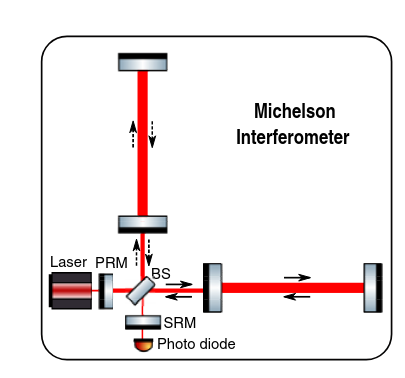
\includegraphics[width=0.35\textwidth, angle=0]{images/IFO.png}
%\caption{Simplified L-shaped interferometer}
%\label{IFO}
%\end{center}
%This image was taken from \cite{Hild_2012}. It depicts the noise source contributions to the advanced LIGO sensitivity curve(left). It highlights the dominance of the quantum noise in the high-frequency region, in contrast to the region below 10Hz, where other noise sources are more dominant(right).
%\end{figure}
%
%\FloatBarrier
%
%Unfortunately, building a detector equally sensitive at all frequencies is currently out of reach of existing instrumental developments. Many types of noise sources make second-generation ground-based gravitational wave detectors most sensitive in the kilohertz band, bounded below by very loud seismic noise and above by quantum noise \cite{Hild_2012}.
%
%\begin{figure}[hbt!]
%\begin{center}
%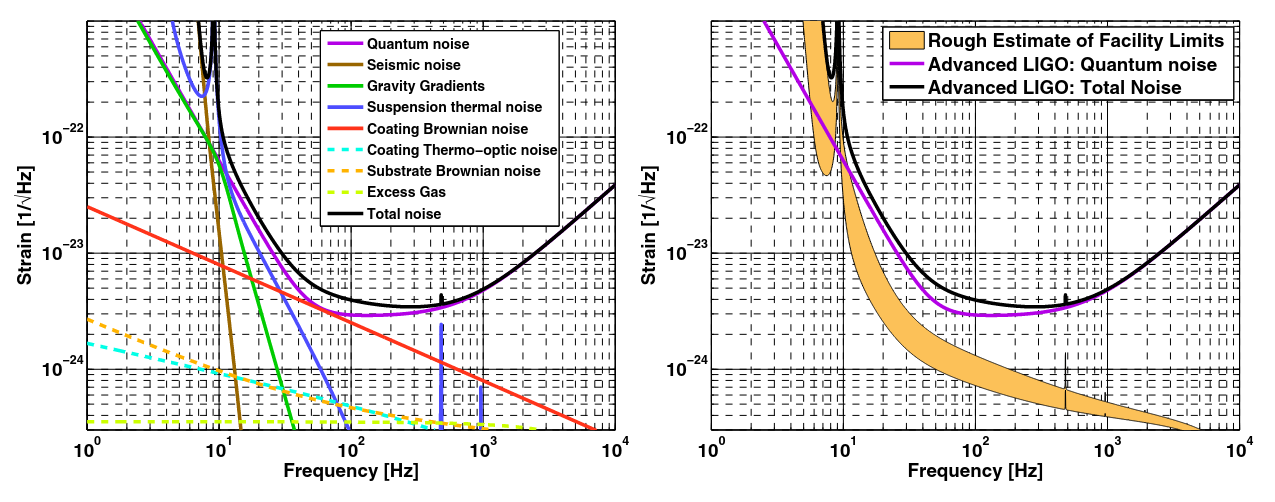
\includegraphics[width=\textwidth, angle=0]{images/aligo.png}
%\caption{LIGO noise sources}
%\label{LIGO}
%\end{center}
%This image was taken from \cite{Hild_2012}. It shows the noise floor of second-generation detectors, its decomposition on different noise sources, and their contribution to the amplitude spectral density of the detector(sensitivity curve).
%\end{figure}
%\FloatBarrier
%
%Even though figure \ref{IFO} shows very simple schematics of Michelson interferometers, in reality, such instruments require huge facilities and cutting-edge technologies to ensure the detector is as sensitive as its components allow. However, not all detectors feature an L-shape configuration. For example  third-generation detectors like LISA and the Einstein telescope will consist of a triangular arrays of mirrors for noise mitigation reasons. 
%
%\begin{figure}[hbt!]
%\begin{center}
%\begin{tabular}{cc}
%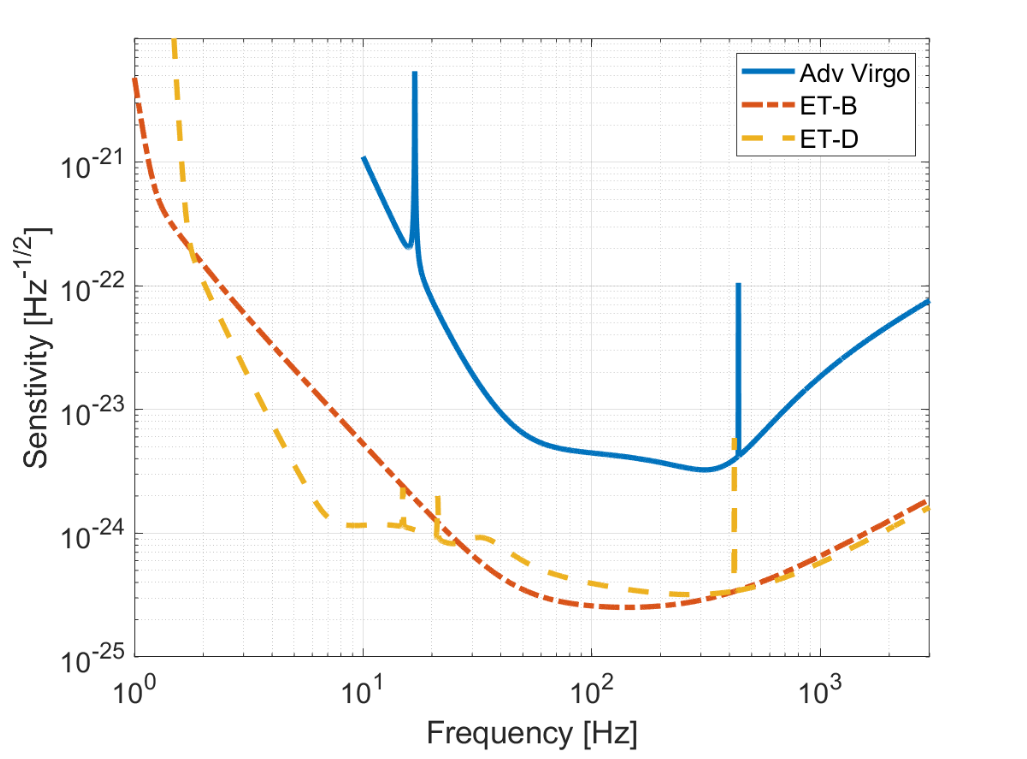
\includegraphics[width=0.5\textwidth, angle=0]{images/ET1.png}
%
%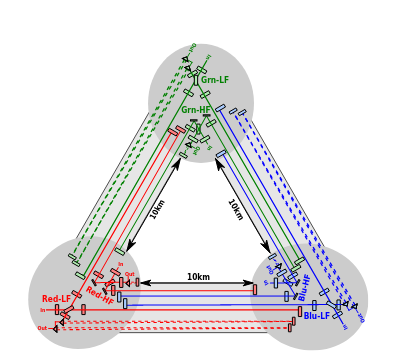
\includegraphics[width=0.5\textwidth, angle=0]{images/ET2.png}
%\end{tabular}
%\end{center}
%\caption{Third generation detectors}
%\label{ET}
%This images were taken from \cite{Maggiore_2020, Sathyaprakash:2011bh}. It shows the sensitivity improvement of the Einstein telescope with respect to VIRGO (left) and shows a scheme of its triangular configuration(right)
%\end{figure}
%\FloatBarrier

 

\chapter{Binary neutron star mergers}

\section{Binary neutron star waveforms}

Section \ref{GW} summarizes the first-order approximation that Einstein himself used to predict the existence of gravitational radiation from Einstein's field equations. However, it falls very short in a more general context, where spacetime perturbations are not weak, nor do the system constituents move in the slow speed approximation regime. Depending on the problem, high-order postnewtonian expansions or numerical relativity simulations have been widely used as our best tool to gain some understanding of several astrophysically relevant scenarios like compact binary mergers and gravitational collapse. 


The physical parameter space of binary neutron star systems is  entirely characterized by the masses of their constituents $m_1$ and $m_2$, their spins $\vec{S}_1$ and $\vec{S}_2$, and their tidal deformabilities s $\Lambda_1$ and $\Lambda2$ \cite{Hinderer:2009ca}. However as current observations are not very sensitive to measuring the individual masses or spins, some other quantities are used in searches.

\begin{equation}\label{chieff}
\chi_{eff} = \frac{m_1}{M}\cdot \chi_1^z + \frac{m_2}{M}\cdot \chi_2^z - \frac{38}{113} \frac{m_1 m_2}{M^2}(\chi_1^z + \chi_2^z)
\end{equation}


\begin{equation}
\tilde{\Lambda} = \frac{16}{13} \left[ \frac{(m_1 +12m_2)(m_1)^4}{M^5} \Lambda^1_2 + \frac{(m_2 +12m_1)(m_2)^4}{M^5} \Lambda^2_2 \right]
\end{equation}

where $\chi_j = \frac{S_j}{m_j}$ is the dimensionless spin parameter, and $\Lambda^j_2 = \frac{2k_2}{3(C_j)^5}$ accounts for the dominant effect of the tidal deformability  which depends on the gravitoelectric love number and the compactness parameter.


\begin{figure}[hbt!]
\begin{center}

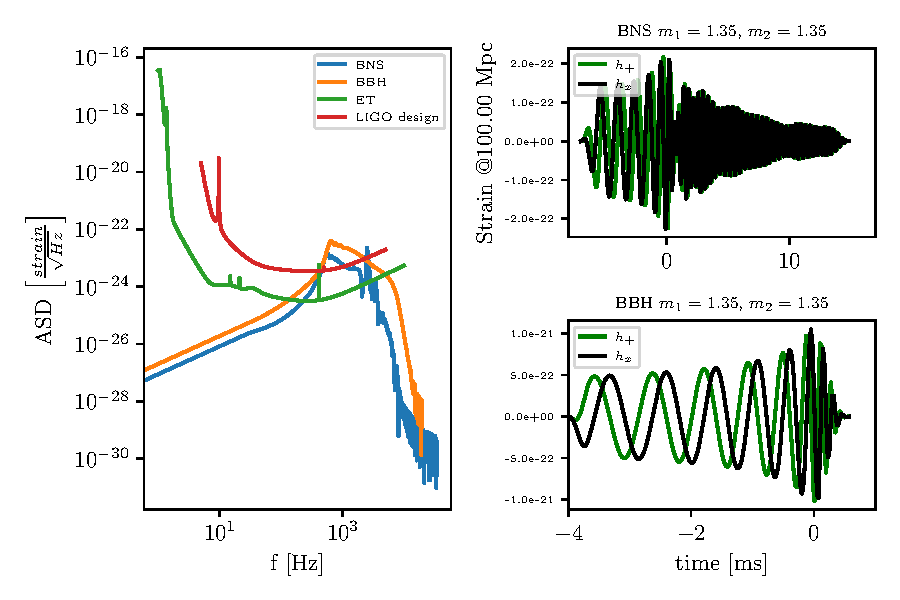
\includegraphics[width=0.7\textwidth, angle=0]{images/Data_analysis/sig_proc/BNS-BBH.pdf}
\caption{BNS and BBH signals in both domains}
\label{BBH and BNS}
\end{center}

Left panel, a magnitude comparison of a BNS signal\cite{Dietrich:2018phi} and BBH signal\cite{Estelles:2020osj} with same progenitor masses against detector sensitivity curves of advanced ligo and Einstein telescope. on the right side, a time domain representation of both signals at 100 megaparsec.

\end{figure}

\FloatBarrier


The two-body problem does not currently have a closed-form solution in general relativity. For example, the merger phase of binary black hole mergers involves self-gravitating systems moving at relativistic speeds while in the presence of their companion's strong gravitational field. In such a regime, postnewtonian approximations can not be applied anymore. 

Binary neutron star and black hole-neutron star systems are much harder to handle during their late inspiral and postmerger phase. Where tidal interactions cause the merger to happen earlier \cite{Hinderer:2009ca, Damour:2009wj,Damour:2012yf}, and the fate and dynamics of the postmerger remnant \cite{Shibata:2019wef} will strongly depend on the equation of state. The equation of state of supranuclear matter is currently unknown, and it would be key in determining:  how each star would deform due to the Tidal field of its companion and how much matter can be supported inside a given spacetime region before collapsing. 

Numerical simulations of these systems have been carried out since 1999-2000 \cite{Shibata:1999hn, Shibata:1999wm}  using the 3+1 decomposition for the spacetime evolution and several different hydrodynamics and magnetohydrodynamics schemes for the matter part of the equations. The gravitational radiation is extracted from those simulations using several methods. Some rely on a spin-weighted spherical harmonic decomposition of the Weyl scalar in coordinate spheres of finite radius \cite{Bishop:2016lgv}, and others use the Cauchy characteristic method to get the radiation field at null infinity \cite{Barkett:2019uae}. 

\begin{equation}
\psi^4 = \ddot{H} = (\ddot{h}_+ - i\ddot{h}_\times) = \sum_{l=-2}^{\infty}  \sum_{m=-l}^{l} {}_{_{_{-2}}}A_{_{_{lm}}}^4 Y_{_{_{lm}}}(\theta, \phi) 
\end{equation}

where the coefficients $A_lm$ are obtained by integrating the weyl scalar over the angular  part 

\begin{equation}
A_{_{_{lm}}} = \oint \psi^4(Y_{_{_{lm}}}(\theta, \phi)) d\Omega
\end{equation}


Where the strain l,m modes can be computed by integrating the weyl scalar multipole coeficients, and the energy and angular momentum carried by the waves can also be computed from them \cite{Ruiz_2007}.

\begin{equation}
h_{lm} = \int dt' dt'' \psi_{lm}^4
\end{equation}

\begin{equation}
\mathcal{E}_{rad} = \lim_{r\to\infty} \frac{c^2 r^2}{16\pi G} \sum_{l=-2}^{\infty}  \sum_{m=-l}^{l} \int_{-\infty}^{t} dt'' \Biggr| \int_{-\infty}^{t''} A_{_{_{lm}}} dt' \Biggr|
\end{equation}

\begin{equation}
\mathcal{E}_{rad} = \lim_{r\to\infty} \frac{c^2 r^2}{16\pi G} \sum_{l=-2}^{\infty}  \sum_{m=-l}^{l} \int_{-\infty}^{t} dt'' \Biggr|  \dot{h}_{_{_{lm}}}(t'')  \Biggr|
\end{equation}


\begin{equation}
\mathcal{J}_{z-rad} = \lim_{r\to\infty} -\frac{i \cdot c^2 r^2}{16\pi G} Im \int_{-\infty}^{t}dt'\left[ \sum_{l=-2}^{\infty} \sum_{m=-l}^{l} m  \left(\int_{-\infty}^{t'} \int_{-\infty}^{t''} dt''dt''' A_{_{_{lm}}}\right)  \cdot \left( \int_{-\infty}^{t'} dt'' (A_{_{_{lm}}})^* \right) \right]
\end{equation}

\begin{equation}
\mathcal{J}_{z-rad} = \lim_{r\to\infty} -\frac{i \cdot c^2 r^2}{16\pi G} Im \int_{-\infty}^{t}dt'\left[ \sum_{l=-2}^{\infty} \sum_{m=-l}^{l} m  \left(h_{lm}\right)  \cdot \left( \dot{h}^*_{lm} \right) \right]
\end{equation}


Gravitational waves computed during such numerical simulations are provided through catalogs as it will be discussed in section \ref{cats}. Unfortunately, existing GW search pipelines need a huge amount of waveforms covering the physical parameter space, which is an unrealizable task to achieve with numerical relativity waveforms.  Currently, BNS searches rely on incomplete semianalytical waveform models based on postnewtonian methods or the effective one-body formalism \cite{Damour:2012yf}. Which have got reasonably good at generating waveforms until the late inspiral phase but do not include any calibrated merger or postmerger oscillations.


\begin{figure}[hbt!]
\begin{center}

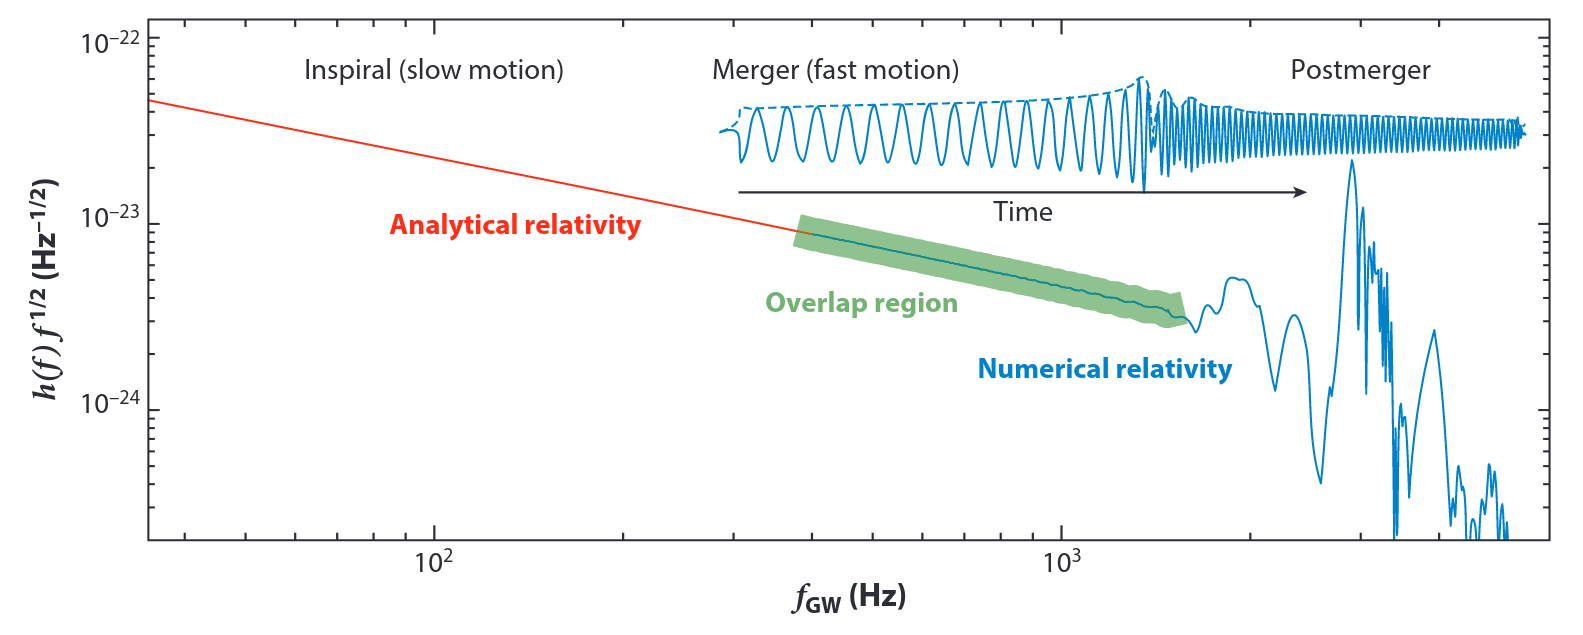
\includegraphics[width=0.6\textwidth, angle=0]{images/postmerger.png}
\caption{BNS waveform: inspiral, merger and postmerger}
\label{BBH and BNS2}
\end{center}
This picture was taken from \cite{Radice_2020}.  It depicts the frequency spectrum of an entire BNS gravitational wave signal, and clearly separates regions where different types of modelling are currently required. 
\end{figure}

\FloatBarrier

\section{Postmerger waveforms}

\section{NR waveform catalogs}





















%\begin{equation}
%\ddot{H} = (\ddot{h}_+ - i\ddot{h}_\times) = \sum_{l=-2}^{\infty}  \sum_{m=-l}^{l} {}_{-2}\psi_{lm}^4 Y_{lm}(\theta, \phi) 
%\end{equation}
%
%\begin{equation}
%h_{lm} = \int dt' dt'' \psi_{lm}^4
%\end{equation}
%
%where one can also define the radiated angular momentum and energy of the waves:
%
%$$
%E = 
%$$
%
%$$
%Jz = 
%$$
%
%In the particular case of binary coalescenses, it may be useful to define several quantities that will act as intrinsic parameters, and are provided as input physics to the simulations. Let $\lambda_1$ and $\lambda2$ [hinderer, nagar]be the tidal deformabilities, $\vec{S}_1$ and $\vec{S}_2$ the spins, and $m_1$ and $m_2$ the masses[][] 
%
%\begin{equation}
%\chi_{eff} = 
%\end{equation}
%
%
%\begin{equation}
%\tilde{\Lambda} = 
%\end{equation}
%
%
%\begin{figure}[hbt!]
%\begin{center}
%
%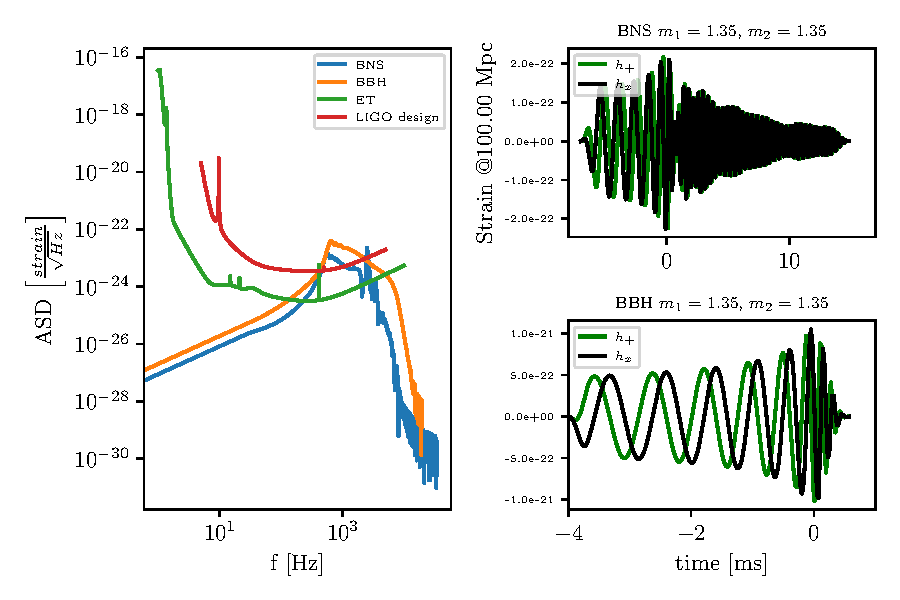
\includegraphics[width=0.9\textwidth, angle=0]{images/Data_analysis/sig_proc/BNS-BBH.pdf}
%\caption{BNS and BBH signals in both domains}
%\label{BBH and BNS}
%\end{center}
%
%Left panel, a magnitude comparison of a BNS signal\cite{Dietrich:2018phi} and BBH signal\cite{Estelles:2020osj} with same progenitor masses against detector sensitivity curves of advanced ligo and Einstein telescope. on the right side, a time domain representation of both signals at 100 megaparsec.
%
%\end{figure}
%
%\FloatBarrier

%\subsection{Waveform models}
%exact solutions to the two body problem in a fully general relativistic context have not been written in closed form. However there the 3+1 decomposition of the Einstein field equations makes the problem suitable for numerical solutions to the spacetime part and the matter part simultaneously, given the Equation of state for the matter present during the colision, except in the case of binary black hole solutions[alcubierre, rezzolla].

